%% Prepared for submission to Knowledge and Information Systems (Springer Nature).
%% NOTE ON TEMPLATE: Springer Nature's own submission guidance for this journal states
%% that LaTeX, Word, or PDF are all accepted at initial submission, and that authors who
%% do not use the official Springer Nature LaTeX template ("sn-jnl.cls") may instead
%% "follow the relevant guide to ensure your manuscript is precisely prepared." This file
%% therefore keeps a correct, freely redistributable, and verified-compilable LaTeX class
%% (elsarticle) as the vehicle, but reformats citations, structure, and metadata to match
%% Springer/KAIS conventions (numbered references, Declarations section, etc.). Before
%% final acceptance, port this content into the official Springer Nature LaTeX template
%% (freely downloadable from Springer Nature's author resources site) and its sn-basic.bst
%% bibliography style; that template file was not fabricated here to avoid introducing an
%% incorrect or outdated proprietary class file.

\documentclass[preprint,12pt]{elsarticle}


\usepackage{amssymb}
%% The amsmath package provides various useful equation environments.
\usepackage{amsmath}
\usepackage{url}
\usepackage{tabularx}
\usepackage{algorithm}
\usepackage{algorithmicx}
\usepackage{algpseudocode}
%% The amsthm package provides extended theorem environments
%% \usepackage{amsthm}

%% The lineno packages adds line numbers. Start line numbering with
%% \begin{linenumbers}, end it with \end{linenumbers}. Or switch it on
%% for the whole article with \linenumbers.
%% \usepackage{lineno}

\begin{document}

\begin{frontmatter}


\title{Retrieval-Assisted Instantiation of Natural-Language Optimization Problems} %% Article title

\author{Soroush Vahidi\corref{cor1}}
\ead{sv96@njit.edu}
\cortext[cor1]{Corresponding author. ORCID: 0000-0003-1934-6282}
\address{Ying Wu College of Computing, New Jersey Institute of Technology, Newark, NJ 07102, USA}

%% NOTE: Knowledge and Information Systems' peer-review blinding policy (single- vs.
%% double-anonymous) could not be confirmed from the publicly accessible Springer Nature
%% pages at the time of this pass -- see the accompanying MANUSCRIPT_README.md. Author
%% identity is included here on the assumption of single-blind review, consistent with
%% the journal's Editorial-Manager-based workflow; confirm at submission and remove the
%% \author/\address block above (leaving only \title and \ead) if double-anonymous review
%% is required.

%% Abstract
\begin{abstract}
Many engineering optimization problems are first described in natural language and only later translated into formal mathematical models, but this translation remains difficult to automate reliably. Rather than targeting full solver-ready generation, this paper studies a narrower intermediate task: retrieval-assisted optimization problem instantiation, viewed as a knowledge-processing problem of grounding natural-language numeric evidence into a structured, typed optimization schema. The contribution is a transparent and reproducible framework that first retrieves the most compatible optimization schema from a fixed catalog and then deterministically instantiates that schema's scalar parameters from numeric evidence in the text, combining lexical schema retrieval, rule-based numeric extraction, coarse type inference, and deterministic compatibility-based slot assignment.

We evaluate the framework on the \textsc{NLP4LP} benchmark of natural-language optimization problems, together with complementary engineering-oriented validation subsets. Schema retrieval is already strong across query variants, with term frequency--inverse document frequency (TF--IDF) retrieval achieving the best average top-1 schema accuracy (Schema R@1 $=0.9094$ on original-text queries). The strongest non-oracle method reaches an InstantiationReady score of $0.5257$, while an oracle upper bound with perfect schema retrieval reaches only $0.5650$: this modest oracle gain shows that the main remaining bottleneck is downstream number-to-slot grounding rather than schema retrieval itself. A pre-fix versus post-fix ablation supports this conclusion: correcting numeric type-handling logic, especially for float-valued slots, yields large improvements in type consistency and query-level readiness. Restricted structural and solver-backed subset studies further suggest downstream optimization-oriented usefulness on compatible cases, without claiming benchmark-wide solver readiness.
\end{abstract}

\begin{keyword}
natural language processing \sep optimization modeling \sep knowledge representation \sep information retrieval \sep semantic grounding \sep intelligent information systems
\end{keyword}

\end{frontmatter}

%% Add \usepackage{lineno} before \begin{document} and uncomment 
%% following line to enable line numbers
%% \linenumbers

%% main text
%%

%% Use \section commands to start a section
\section{Introduction}

\subsection{Background and Motivation}
\label{subsec:intro_background}

Many real-world engineering and operations problems are first described in natural language before they are formalized as optimization models. Analysts, planners, and domain experts often specify resource limits, costs, capacities, proportions, and operational rules in text long before these elements are translated into a mathematical program. This gap between informal problem descriptions and formal optimization artifacts has motivated growing interest in natural-language interfaces for optimization, including benchmark datasets, assistive formulation systems, and more recent large-language-model-based pipelines \cite{ramamonjison2022autoformulation,ramamonjison2023nl4opt,ahmaditeshnizi2024optimus_icml,zhang2024optllm,huang2024llmoptimization}. The problem is important not only from the perspective of automation, but also for engineering decision support: a system that can reliably connect a textual problem description to an appropriate optimization structure can reduce modeling effort, improve accessibility, and support practitioners during early stages of formalization.

At the same time, full natural-language-to-optimization translation remains difficult. A complete system must determine which optimization template or problem class is appropriate, identify the relevant quantities mentioned in text, align these quantities with the correct model parameters, and ultimately produce a formulation that is structurally and numerically usable. Recent work has shown that large language models and related systems can generate optimization-oriented code, formulations, or solver inputs from text \cite{ahmaditeshnizi2024optimus_icml,zhang2024optllm,ahmed2025opt2code,ramamonjison2023latex2solver,singirikonda2025text2zinc}. However, such end-to-end settings combine several sources of difficulty at once, making it hard to determine which intermediate capabilities are reliable, which stages contribute most to failure, and which parts of the pipeline already provide practical value for engineering optimization workflows.

This paper adopts a narrower and more transparent perspective. Rather than attempting to generate a complete solver-ready optimization model from text, we focus on an intermediate task that is both practically meaningful and experimentally tractable: given a natural-language optimization description, can a deterministic system retrieve the most compatible optimization schema and then instantiate its scalar parameters from textual numeric evidence? This perspective is motivated by two observations. First, schema retrieval is a necessary prerequisite for many downstream modeling pipelines because parameter interpretation depends on the underlying problem structure. Second, partial but reliable recovery of scalar parameters can still provide useful modeling support even when full formulation generation remains out of reach. In this sense, retrieval-assisted schema grounding can be viewed as a transparent decision-support layer between free-form language and formal optimization artifacts.

This framing is especially relevant for engineering-oriented AI support. In contrast to opaque end-to-end generation, a retrieval-assisted deterministic pipeline exposes its intermediate decisions: which schema was selected, which scalar slots were considered eligible, which numeric mentions were extracted, and how assignments were made. Such transparency is valuable in optimization settings, where users often need to inspect, verify, and revise system outputs before trusting them in a modeling workflow. Related work on explainable and user-facing optimization systems similarly emphasizes the importance of interpretability, usability, and human-centered support around optimization technology \cite{biemans2025explainableoptimization,powell2025scheduling_explanations}. Our goal is therefore not to replace the modeling expert, but to study whether a simple, reproducible, retrieval-centered system can provide measurable downstream utility for structured optimization problem instantiation.

Guided by this motivation, we study a deterministic retrieval-assisted framework on the \textsc{NLP4LP} benchmark \cite{nlp4lp_dataset,ahmaditeshnizi2024optimus_icml}. The framework first retrieves a candidate schema from a fixed catalog and then performs deterministic scalar parameter instantiation conditioned on the retrieved schema. This restricted formulation allows us to ask a focused question: how much structured downstream utility can be obtained from transparent lexical retrieval and deterministic number-to-slot grounding alone, before introducing learned retrievers, large language models, or more complex solver-coupled components? As the experiments later show, this question is useful precisely because it separates two issues that are often conflated in end-to-end systems: retrieving the correct broad problem structure and grounding the numerical content of the query into the correct scalar roles. The remainder of the introduction positions this perspective relative to prior work, clarifies the scope of the paper, and summarizes the main contributions.

\subsection{Related Work}
\label{subsec:intro_related}

Research at the intersection of natural language processing and optimization has expanded rapidly in recent years. An important early direction has focused on helping users convert textual problem descriptions into formal optimization artifacts. Ramamonjison et al.\ introduced an assistive auto-formulation framework in which natural-language problem descriptions are mapped to editable optimization-model suggestions, combining automatic support with interactive modeling assistance \cite{ramamonjison2022autoformulation}. This line of work also led to benchmark-oriented efforts such as \textsc{NL4Opt}, which helped establish natural-language-to-optimization as a shared evaluation problem and emphasized the extraction of optimization entities and machine-interpretable structure from text \cite{ramamonjison2023nl4opt}. Related work such as \textsc{LaTeX2Solver} explored hierarchical parsing pipelines for converting semi-structured mathematical documents into optimization-oriented code representations \cite{ramamonjison2023latex2solver}. Together, these studies demonstrate both the importance of the problem and the diversity of interfaces between language and optimization.

A second and increasingly prominent direction uses large language models for end-to-end optimization modeling. \textsc{OptiMUS} studies how large language models, together with solver feedback, can formulate, implement, debug, and solve linear and mixed-integer programming problems from natural-language descriptions \cite{ahmaditeshnizi2024optimus_icml,ahmaditeshnizi2024optimus03}. OptLLM likewise proposes an LLM-centered framework augmented with external solvers for converting natural-language optimization requests into formulations, code, and solutions \cite{zhang2024optllm}. More recently, retrieval-augmented generation has also been explored in this setting. \textsc{OPT2CODE}, for example, combines retrieval, code generation, and judge-based checking to translate linear-programming descriptions into solver-executable code \cite{ahmed2025opt2code}. These systems have advanced the state of the art in end-to-end automation, but they also combine several difficult subproblems at once, including problem understanding, formulation generation, numerical grounding, code production, and downstream validation.

Beyond full model generation, several works have examined intermediate components of the language-to-optimization pipeline. \textsc{Ner4Opt} frames optimization modeling support as an information-extraction problem over natural-language descriptions, focusing on optimization-relevant entities and quantities needed for downstream modeling \cite{kadioglu2024ner4opt}. Recent benchmark work has also broadened the scope beyond linear and mixed-integer programming. For example, \textsc{Text2Zinc} introduces a cross-domain dataset for optimization and satisfaction problems in \textsc{MiniZinc}, while \textsc{CP-Bench} evaluates large language models for constraint modeling across multiple constraint-programming systems \cite{singirikonda2025text2zinc,michailidis2025cpbench}. Related work such as \textsc{EHOP} further shows that the linguistic presentation of optimization-style tasks can materially affect model performance, reinforcing the value of studying intermediate language-to-structure capabilities directly \cite{duchnowski2025ehop}. At a broader level, recent surveys and position papers document the rapidly growing interaction between large language models and optimization, including both using optimization to improve language models and using language models to support optimization workflows \cite{huang2024llmoptimization,huang2025llmsmathmodeling}.

Another nearby strand of work concerns explainability and human-centered support for optimization systems. Rather than generating optimization models from text, these approaches use language models to explain schedules, decisions, or optimization outcomes in user-friendly terms \cite{biemans2025explainableoptimization,powell2025scheduling_explanations}. This perspective is relevant to engineering decision support because it emphasizes transparency, trust, and usability in optimization-assisted workflows. However, it addresses a different stage of the pipeline: explaining optimization outputs rather than grounding natural-language problem descriptions into formal model structure.

Our work is most closely related to natural-language-to-optimization modeling, but it occupies a different point in the design space from both end-to-end generation systems and component-level extraction systems. In contrast to approaches that aim to produce complete formulations, executable code, or solver-ready models, we focus on a narrower intermediate task: retrieval-assisted schema grounding followed by scalar parameter instantiation. In contrast to pure extraction approaches, we make downstream slot eligibility depend explicitly on the retrieved schema, so that downstream evaluation remains structurally tied to schema selection quality. This design allows us to isolate an empirically important question that is often obscured in end-to-end pipelines: whether the main difficulty lies in retrieving the correct broad optimization structure or in grounding the numerical content of the query into the correct scalar roles once that structure has been identified.

The resulting perspective places the paper between full automation and low-level entity extraction. The proposed framework is fully deterministic and transparent, which makes it possible to analyze where gains arise and where residual errors remain. More importantly, it allows us to evaluate a practically meaningful intermediate capability for engineering optimization support without conflating it with full formulation synthesis. In particular, our experiments show that lexical schema retrieval on \textsc{NLP4LP} is already strong, whereas the main remaining bottleneck is downstream number-to-slot grounding. We therefore position this paper as a study of retrieval-assisted optimization-model support: not full natural-language-to-optimization compilation, but schema retrieval and schema-conditioned scalar instantiation as measurable and practically useful components of a broader engineering decision-support workflow.


\subsection{Problem Scope and Proposed Perspective}
\label{subsec:intro_scope}

The present study focuses on a deliberately restricted but practically meaningful intermediate task in natural-language-to-optimization. Rather than attempting to translate a problem description directly into a complete solver-ready formulation, we study whether a system can first retrieve an appropriate optimization schema and then recover the scalar quantities needed to instantiate that schema. This perspective reflects an important modeling reality: before variables, objectives, and constraints can be finalized, a system must determine which broad problem template is relevant and how the numerical evidence in the text should be aligned with the parameter structure of that template. By isolating this intermediate stage, we can evaluate a core component of optimization-oriented language understanding without conflating it with the additional complexity of full formulation synthesis.

Our formulation is intentionally retrieval-centered. Given a natural-language query, the system ranks a fixed catalog of candidate schemas and selects the top-ranked template as the predicted problem structure. The retrieved schema is then used to determine which scalar parameter slots are eligible for instantiation, after which deterministic rules assign numeric mentions extracted from the query to those slots. This design makes the second stage explicitly dependent on the first: if schema retrieval is incorrect, the downstream parameter space may also be incorrect, even when the query still contains informative numeric evidence. In this sense, retrieval is not merely a preprocessing step; it is the structural grounding mechanism that connects free-form language to an optimization template.

This paper therefore adopts a narrower scope than end-to-end natural-language-to-optimization systems. The main benchmarked task is schema-conditioned scalar parameter instantiation: the framework does not attempt to synthesize a complete mathematical program, enumerate all variables and constraints, or recover structured parameter objects such as lists, vectors, or dictionaries at benchmark scale. These restrictions are deliberate. They allow the core study to concentrate on a transparent and reproducible question: how much downstream structured utility can be obtained from deterministic schema retrieval and scalar parameter instantiation alone? In this setting, strong benchmark performance should be interpreted as evidence of useful schema grounding and partial parameter recovery, not as complete optimization-model generation.

At the same time, this restricted formulation does not imply that the paper is disconnected from practical engineering use. In addition to the main benchmark study, we include downstream engineering-oriented validation on restricted subsets, including structural-validity analysis and a small solver-backed executable study on compatibility-filtered instances. These additional experiments do not change the core task definition, but they help assess whether retrieval-assisted scalar instantiation can support later stages of optimization modeling in practice. Accordingly, the paper should be read as a study of an intermediate capability with downstream engineering relevance, rather than as a claim of full benchmark-wide solver-ready automation.

This perspective also motivates the evaluation design of the paper. Because eligible slots are determined from the predicted schema rather than the gold schema, downstream performance remains retrieval-dependent by construction. As a result, the experiments can measure not only whether the correct template is retrieved, but also whether improved retrieval translates into better structured parameter recovery. The final benchmark results make this distinction especially informative: schema retrieval on \textsc{NLP4LP} is already strong, whereas the main remaining difficulty lies in grounding extracted numeric evidence to the correct scalar roles once a plausible schema has been identified. This evaluation-oriented formulation is therefore central to the contribution of the paper. It makes it possible to study schema retrieval and scalar instantiation in their own right, while preserving a clear connection between retrieval quality and downstream utility.

Within this scope, we propose a fully deterministic framework based on lexical schema retrieval and rule-based parameter grounding. This choice is intentional. Recent literature has shown that large language models and retrieval-augmented systems can generate optimization code, formulations, or solver-oriented outputs from text \cite{ahmaditeshnizi2024optimus_icml,zhang2024optllm,ahmed2025opt2code,ramamonjison2023latex2solver}, but such systems combine many modeling, grounding, and verification challenges at once. By contrast, our framework is designed to expose each intermediate decision and thereby support closer analysis of what transparent retrieval and deterministic grounding can already achieve. This positions the paper between full automation and low-level extraction: the proposed system is neither a complete natural-language-to-optimization compiler nor a purely local entity recognizer, but a transparent retrieval-assisted instantiation pipeline intended to quantify the downstream value of schema grounding.

In summary, the proposed perspective is to treat optimization schema retrieval and scalar parameter instantiation as a standalone intermediate problem with clear relevance to engineering optimization support. This framing is narrow enough to permit precise evaluation and error analysis, yet broad enough to capture an important step in the pathway from informal language to formal optimization models. The next subsection summarizes the main contributions of the paper and outlines the organization of the remainder of the manuscript.

\subsection{Contributions and Engineering-AI Implications}
\label{subsec:intro_contributions}

This paper makes six main contributions. First, it decomposes natural-language optimization understanding into two explicit, separately measurable stages: schema retrieval and schema-conditioned scalar parameter grounding, connected by a retrieval-dependent evaluation design in which eligible parameter slots are determined by the predicted schema rather than the gold schema. Second, it proposes a transparent, deterministic framework for mapping numeric textual evidence to typed optimization-schema parameters, combining lexical schema retrieval, rule-based numeric extraction, coarse type inference, and no-reuse compatibility-based slot assignment; the resulting pipeline is reproducible and inspectable at every intermediate step. Third, it introduces optimization-role and admissibility reasoning -- a deterministic, lexicon-based refinement layer that scores slot--mention compatibility using role cues (e.g., capacity, cost, or cardinality-bound language) in addition to coarse type agreement -- and reports its measured effect relative to the simpler typed-greedy baseline. Fourth, it provides a controlled empirical comparison, supported by paired bootstrap significance testing, showing that downstream grounding -- not schema retrieval -- is the dominant bottleneck: an oracle upper bound with perfect schema retrieval improves \textit{InstantiationReady} only from $0.5257$ to $0.5650$, a small and statistically significant but practically modest gain. Fifth, it reports structural and restricted solver-backed validation (a 60-instance structural subset, a 269-instance executable-attempt subset, and a 20-instance Gurobi-free solver-backed subset) that clearly distinguishes what is reproducible end-to-end from what remains unsupported at benchmark scale. Sixth, it provides a detailed error and failure analysis -- an error taxonomy, a pre-fix versus post-fix ablation of numeric type handling, and a negative result for three additional deterministic grounding families (global-compatibility, relation-aware, and ambiguity-aware grounding) -- that identifies semantic quantity-to-role ambiguity as the primary target for future hybrid learned/constrained grounding methods.

Beyond these technical contributions, the paper has a broader implication for engineering AI support. In many operational settings, the practical goal is not immediate full automation, but the development of tools that help users move from informal descriptions to formal decision models in a controlled and inspectable way. From this perspective, retrieval-assisted schema grounding is useful because it narrows the candidate modeling space, exposes the inferred template structure, and provides partial parameter recovery that can be checked, corrected, or extended by a human decision maker. This emphasis on transparency, traceability, and human oversight is consistent with recent work on explainable and user-facing optimization support \cite{biemans2025explainableoptimization,powell2025scheduling_explanations}.

The empirical findings should be interpreted in this spirit. The proposed system is not presented as a complete natural-language-to-optimization compiler, nor as a replacement for an optimization modeler. Instead, it is studied as a transparent intermediate layer that quantifies how much useful structure can be recovered through deterministic retrieval and assignment, and how far such recovery can support downstream engineering-oriented validation. The results show that lexical schema retrieval on \textsc{NLP4LP} is already strong, whereas the main remaining bottleneck lies in downstream number-to-slot grounding under semantic ambiguity. This perspective complements recent large-language-model-based optimization systems by clarifying what can already be achieved with a transparent pipeline and where stronger downstream reasoning is still needed \cite{ahmaditeshnizi2024optimus_icml,zhang2024optllm,ahmed2025opt2code}.

The remainder of the paper is organized as follows. Section~\ref{sec:method} presents the problem formulation, retrieval stage, deterministic parameter-instantiation backbone, and evaluation-oriented design choices. Section~\ref{sec:experiments} describes the experimental setup and reports retrieval performance, downstream utility, engineering-oriented validation, and error analysis. Section~\ref{sec:conclusion} concludes with the main findings, limitations, and directions for future work.

\section{Methodology}
\label{sec:method}

\subsection{Problem Formulation}
\label{subsec:method_problem}

We study a retrieval-assisted instantiation task for natural-language optimization descriptions. Given a query that describes an optimization problem, the objective is not to generate a complete mathematical program directly. Instead, the system produces two structured outputs: (i) a schema prediction that identifies the most compatible optimization template from a fixed catalog, and (ii) scalar parameter assignments for the retrieved schema. This formulation captures an important intermediate step in natural-language-to-optimization pipelines: before a full model can be constructed, the system must identify an appropriate template and recover the key quantities needed to instantiate it \cite{nlp4lp_dataset,ramamonjison2023nl4opt,ahmaditeshnizi2024optimus_icml}.

We cast the task as a two-stage decision process. In the first stage, the system performs \emph{schema retrieval}: given a query $q$, it ranks a catalog $\mathcal{S}=\{s_1,\dots,s_M\}$ of candidate optimization schemas and returns the top-ranked schema
\[
\hat{s}=\arg\max_{s \in \mathcal{S}} \mathrm{score}(q,s).
\]
Each schema represents an optimization template together with its associated parameter structure. In the second stage, the system performs \emph{parameter instantiation}: conditioned on the retrieved schema $\hat{s}$, it extracts numeric mentions from the query and assigns them to the scalar parameter slots specified by $\hat{s}$ using deterministic grounding rules. The second stage is explicitly retrieval-dependent: if schema retrieval is incorrect, the set of eligible parameter slots may also be incorrect, reducing downstream coverage and readiness even when the query still contains informative numeric evidence.

In this paper, the term \emph{schema} refers to the retrieved optimization template together with the scalar parameter structure to be instantiated. The resulting task is narrower than full natural-language-to-optimization translation. The main benchmarked setting does not attempt to synthesize a complete optimization model, recover all variables and constraints, or reconstruct structured parameter objects such as lists, vectors, or dictionaries. Rather, the focus is on whether schema retrieval can anchor a natural-language description to a plausible optimization template, and whether deterministic grounding can recover useful scalar values once that template has been selected.

Our scope is intentionally restricted in three ways. First, benchmark-level downstream evaluation is limited to scalar numeric parameters. Second, the core retrieval-and-grounding pipeline is fully deterministic and uses no large language model, no learned retriever, and no learned extractor. Third, the main benchmark study evaluates schema-conditioned scalar recovery rather than full end-to-end model generation. These restrictions are deliberate: they isolate an interpretable intermediate capability and allow precise analysis of where performance gains and failures arise. At the same time, the broader experimental section complements this benchmarked formulation with engineering-oriented subset validation, including structural-validity analysis and a restricted solver-backed study on compatible instances. These additional experiments are intended to assess downstream practical relevance, not to redefine the core task studied here.

Formally, let $G(q)$ denote the set of scalar gold parameters associated with query $q$, and let $P(\hat{s})$ denote the scalar parameter keys exposed by the retrieved schema $\hat{s}$. The downstream evaluator considers only the eligible slot set
\[
E(q,\hat{s}) = G(q) \cap P(\hat{s}),
\]
that is, the scalar gold parameters whose keys are present in the predicted schema. This choice makes downstream evaluation retrieval-dependent by construction. Even when a query contains the correct numeric evidence, an incorrect schema can reduce structural overlap and therefore lower downstream performance. The formulation is designed to measure not only whether the correct schema is retrieved, but also whether improved schema retrieval yields measurable gains in structured parameter instantiation.

Retrieval quality is measured by whether the top-ranked schema matches the gold schema, while downstream quality is measured by how well scalar slots from the retrieved schema can be instantiated from the query text. As the experiments later show, retrieval on \textsc{NLP4LP} is already strong, whereas the main remaining difficulty lies in grounding extracted numbers to the correct scalar roles within the chosen schema. The formulation adopted here therefore isolates the stage that currently matters most empirically: deterministic number-to-slot grounding after schema retrieval.

\subsection{Retrieval-Based Schema Identification}
\label{subsec:method_retrieval}

The first stage of the framework performs \emph{schema identification by retrieval}. Given a natural-language optimization description, the system selects the most compatible candidate from a fixed catalog of benchmark-induced schema documents. We formulate this stage as a ranking problem over a finite candidate set $\mathcal{S}$. Each candidate document is indexed by a schema identifier and paired with the textual schema description used by the evaluation pipeline. Given an input query, the retriever scores the query against every candidate document and returns a ranked list. In the present pipeline, only the highest-ranked candidate is used, so retrieval is treated as a top-1 schema selection problem rather than a shortlist-generation or interactive retrieval task.

It is important to clarify what a ``schema candidate'' means in this setting. The retrieval corpus is the benchmark-induced catalog used by the current evaluation pipeline, and in the repository rerun it contains 335 candidate schema documents. Thus, the retrieval task in this paper is neither open-domain optimization search nor coarse classification into a small number of broad problem families. Instead, it is a fixed-catalog identification problem: for each query, the system must select the single benchmark schema document that serves as the structural template for downstream grounding. This benchmark-specific formulation is deliberate because the goal of the paper is to study whether natural-language optimization descriptions can first be anchored to a usable template and then instantiated deterministically.

Operationally, the retrieved schema serves as the structural anchor for downstream instantiation. Through its identifier, the system accesses the associated parameter structure and uses that structure to determine which scalar slots are eligible for filling. The retrieval stage therefore does \emph{not} attempt to reconstruct a full symbolic optimization model, derive solver-ready constraints, or generate variables and objectives directly. Instead, it selects the most plausible template index from which the downstream stage can obtain an expected set of scalar parameter roles \cite{nlp4lp_dataset,ramamonjison2023nl4opt,ahmaditeshnizi2024optimus_icml}.

This fixed-catalog setup should also be distinguished from label-only classification. The retriever does not predict an abstract class name from a small closed set of manually engineered categories. Rather, it ranks textual schema documents using their natural-language content. This distinction matters because the empirical question in our benchmark is not merely whether a query belongs to a broad optimization family, but whether it can be aligned to the \emph{specific} schema document whose parameter inventory is then used for downstream slot grounding. Retrieval quality therefore directly affects the structural conditions under which the second stage operates.

We evaluate three deterministic lexical retrieval baselines: BM25 \cite{robertson2009bm25}, TF--IDF cosine retrieval \cite{pedregosa2011sklearn}, and latent semantic analysis (LSA) \cite{deerwester1990lsa}. All three retrievers are deterministic, CPU-based, and operate directly on schema-catalog text without benchmark-specific training, dense neural encoders, or learned reranking. Table~\ref{tab:retrieval_backbones} summarizes their roles in the pipeline.

For a query $q$, each retriever produces a score for every candidate schema $s \in \mathcal{S}$, and the predicted schema is
\begin{equation}
\hat{s}(q) = \arg\max_{s \in \mathcal{S}} \mathrm{score}(q,s).
\label{eq:schema_retrieval}
\end{equation}
Only $\hat{s}(q)$ is passed to the downstream instantiation stage. This top-1 design matches the evaluation goal of the paper: we ask whether the system can identify a single usable schema that supports deterministic slot filling, rather than whether it can produce a longer candidate list for later interaction or reranking.

To interpret retrieval performance, we use two diagnostic references in the broader pipeline. The first is an \emph{oracle} control, which replaces the retrieval output with the gold schema identifier and therefore exposes downstream behavior under perfect schema selection. The second is a \emph{random} reference. For retrieval-only evaluation, this random reference is the theoretical top-1 chance rate under uniform selection over the 335 candidate schema documents used in the current rerun, namely $1/335 \approx 0.0030$. For downstream evaluation, ``random'' instead denotes a uniformly chosen schema passed through the same deterministic instantiation pipeline. These references are included only to calibrate interpretation; they are not competing learned retrievers.

Because the retrieved schema determines the candidate slot inventory used downstream, retrieval errors propagate structurally. If the wrong schema is selected, the second stage may inherit a slot set that only partially overlaps the gold instance or that mismatches the intended scalar roles altogether. This can reduce downstream coverage, type agreement, and per-query readiness even when the query still contains relevant numeric evidence. Conversely, strong retrieval creates more favorable structural conditions for deterministic grounding by supplying a more appropriate set of candidate slots.

This formulation emphasizes retrieval as \emph{schema grounding} rather than full optimization-model reconstruction. The purpose of the first stage is to map a free-form optimization description to a single candidate template whose scalar parameter structure can then be instantiated transparently. As the experiments later show, schema retrieval on \textsc{NLP4LP} is already strong, especially for TF--IDF, while the main remaining difficulty lies downstream in number-to-slot grounding. Retrieval is therefore an important enabling step in the pipeline, but not the dominant empirical bottleneck in the current benchmark setting.

\begin{table}[t]
\centering
\caption{Deterministic retrieval backbones used for schema identification.}
\label{tab:retrieval_backbones}
\small
\begin{tabularx}{\linewidth}{l l X}
\hline
Method & Representation & Role in pipeline \\
\hline
BM25 & Probabilistic lexical weighting & Sparse lexical baseline \\
TF--IDF & Weighted bag-of-words cosine similarity & Main deterministic retrieval backbone \\
LSA & Latent projection of TF--IDF features & Lower-dimensional lexical-semantic baseline \\
\hline
\end{tabularx}
\end{table}

\subsection{Deterministic Parameter Instantiation}
\label{subsec:method_instantiation}

Given a natural-language query and a predicted schema, the second stage of the framework instantiates scalar parameter slots from textual numeric evidence. The output of this stage is a set of slot--value assignments associated with the retrieved schema. In the main benchmarked setting, this stage does not generate a complete optimization model and does not recover variables, constraints, or structured parameter objects. Its purpose is narrower: to recover scalar values that can be aligned with the parameter structure of the retrieved template.

The instantiation stage begins by extracting candidate numeric mentions from the query text using a fixed rule-based pattern matcher. The extractor recognizes integers, decimals, percentage expressions, currency-like forms, and comma-separated magnitudes. In degraded query settings, masked placeholders are preserved as special tokens but treated as numerically unknown, so they cannot support exact value recovery. Each extracted mention is then assigned a coarse type label from four buckets: \emph{percent}, \emph{integer}, \emph{currency}, and \emph{float}. Mention typing relies on deterministic surface cues such as percentage markers, currency markers, integer-valued forms, and local lexical context.

The predicted schema determines which parameter slots are eligible for instantiation. Operationally, the system obtains the parameter keys associated with the retrieved template and then restricts attention to scalar-valued slots. This restriction is deliberate. List-valued and dictionary-valued parameters correspond to more structured objects whose recovery would require additional representational assumptions, so the present framework focuses on scalar numeric instantiation. The instantiation problem is therefore defined over a finite set of eligible scalar slots together with a pool of extracted numeric candidates.

For each eligible slot, an expected type is inferred from its parameter name using deterministic rules. Parameters whose names indicate rates or fractions are mapped to \emph{percent}; names indicating counts or cardinalities are mapped to \emph{integer}; names suggesting monetary quantities are mapped to \emph{currency}; and all remaining scalar slots are mapped to \emph{float}. This shared typed representation places slots and extracted numeric mentions in a common compatibility space before assignment.

The simplest assignment rule used in the framework is typed greedy matching. Let $\mathcal{P}=\{p_1,\dots,p_m\}$ denote the eligible scalar slots induced by the predicted schema, and let $\mathcal{T}=\{t_1,\dots,t_n\}$ denote the extracted numeric mentions. In the typed-greedy setting, the selected mention for slot $p_i$ is the highest-scoring unused candidate under a deterministic compatibility rule,
\begin{equation}
t_i^{*} = \arg\max_{t \in \mathcal{T}\setminus \mathcal{U}_{i-1}} \mathrm{compat}(p_i,t),
\label{eq:typed_assignment}
\end{equation}
where $\mathcal{U}_{i-1}$ is the set of mentions already assigned in previous steps. The compatibility function prioritizes agreement between the expected slot type and the inferred mention type, together with deterministic tie-breaking based on local cues and extraction order. Once a mention is assigned, it is removed from the candidate pool and cannot be reused for later slots. This yields a one-pass deterministic assignment rule rather than a global combinatorial optimizer.

The broader method family evaluated in the paper extends this same backbone. In addition to lexical typed-greedy baselines, we consider deterministic grounding variants that modify how slot--mention compatibility is scored or revised after an initial assignment. These include constrained matching, semantic repair, optimization-role repair, acceptance reranking, hierarchical acceptance reranking, and the newer relation-aware, global-compatibility, and ambiguity-aware variants introduced in the updated rerun. Although these methods differ in scoring or repair strategy, they share the same core structure: deterministic numeric extraction, schema-conditioned scalar slot selection, coarse type inference, and no-reuse slot filling. This common backbone is summarized in Algorithm~\ref{alg:instantiation} and illustrated in Figure~\ref{fig:instantiation-pipeline}.

We use \emph{optimization-role compatibility} to refer to a deterministic, lexicon-based refinement of the basic type-compatibility signal used by \texttt{tfidf\_optimization\_role\_repair} and the newer relation-aware and global-compatibility variants. Beyond the coarse type label (\emph{percent}, \emph{integer}, \emph{currency}, \emph{float}), each slot name and its local query context are matched against a fixed lexicon of optimization-role cue words (e.g., terms indicating a capacity limit, a cost coefficient, a cardinality bound, or a derived count). When a candidate mention's local context shares a role cue with the slot, the deterministic assignment score in Eq.~\eqref{eq:typed_assignment} receives an additive bonus; when the mention's inferred type is incompatible with the slot's expected type, it receives a penalty large enough to make the mention non-preferred (though not strictly inadmissible, since ties and missing alternatives can still cause an incompatible mention to be assigned). We use \emph{admissibility} in this paper only in this graded, score-based sense -- a slot--mention pairing is more or less preferred under the compatibility rule -- rather than as a hard combinatorial constraint verified against a formal model of the optimization problem; the framework does not currently guarantee that an admissible-by-type assignment is also feasible or optimal for the underlying (unobserved) mathematical program. This is a heuristic, rule-based layer, and we report it as such: it is designed to break ties among type-compatible candidates using domain-typical lexical cues, not to provide a formal correctness guarantee.

To isolate the effect of type-aware matching, we also evaluate a pre-fix versus post-fix comparison of the typed compatibility logic. The key issue addressed by the post-fix implementation is the handling of \emph{float}-valued slots, whose compatibility with extracted numeric mentions was previously underestimated by the type-matching logic. As the experiments later show, correcting this behavior materially improves \textit{TypeMatch} and \textit{InstantiationReady} while leaving extraction-dependent quantities much less changed. This confirms that the main downstream gains arise from improved number-to-slot grounding rather than from changes in retrieval or mention extraction.

In short, the instantiation stage is intentionally simple: numeric evidence is extracted from the query, typed using deterministic cues, filtered through the scalar parameter structure of the predicted schema, and assigned to slots by a deterministic no-reuse procedure. The resulting slot--value mapping is then evaluated downstream. In the broader paper, this benchmarked scalar-instantiation stage is complemented by restricted engineering-oriented validation on subsets, but the core methodology here remains a deterministic, schema-conditioned scalar grounding pipeline.

\begin{algorithm}[t]
\caption{Deterministic parameter instantiation pipeline. Numeric mentions are extracted from the query and typed using surface cues. In parallel, the predicted schema provides the eligible scalar slots, whose expected types are inferred from slot names. A deterministic compatibility-based assignment procedure then maps numeric mentions to slots without token reuse. Different downstream variants share this backbone but differ in how slot--mention compatibility is scored or repaired.}
\label{alg:instantiation}
\small
\begin{algorithmic}[1]
\Require Query text $q$, predicted schema $\hat{s}$
\Ensure Slot--value mapping $A$
\State Extract numeric mentions $\mathcal{T}$ from $q$
\State Infer a coarse type for each mention in $\mathcal{T}$
\State Obtain parameter keys from schema $\hat{s}$
\State Restrict to eligible scalar slots $\mathcal{P}=\{p_1,\dots,p_m\}$
\State Infer an expected type for each slot in $\mathcal{P}$
\State Initialize assignments $A \leftarrow \emptyset$ and used-mention set $\mathcal{U}\leftarrow \emptyset$
\For{each slot $p_i \in \mathcal{P}$}
    \State Define candidate set $\mathcal{C}_i \leftarrow \mathcal{T} \setminus \mathcal{U}$
    \If{$\mathcal{C}_i = \emptyset$}
        \State \textbf{continue}
    \EndIf
    \State Score mentions in $\mathcal{C}_i$ using a deterministic slot--mention compatibility rule
    \State Select the highest-ranked mention $t_i^{*}$
    \State Assign $A[p_i] \leftarrow \mathrm{value}(t_i^{*})$
    \State Update $\mathcal{U} \leftarrow \mathcal{U} \cup \{t_i^{*}\}$
\EndFor
\State \Return $A$
\end{algorithmic}
\end{algorithm}

\begin{figure}[t]
  \centering
  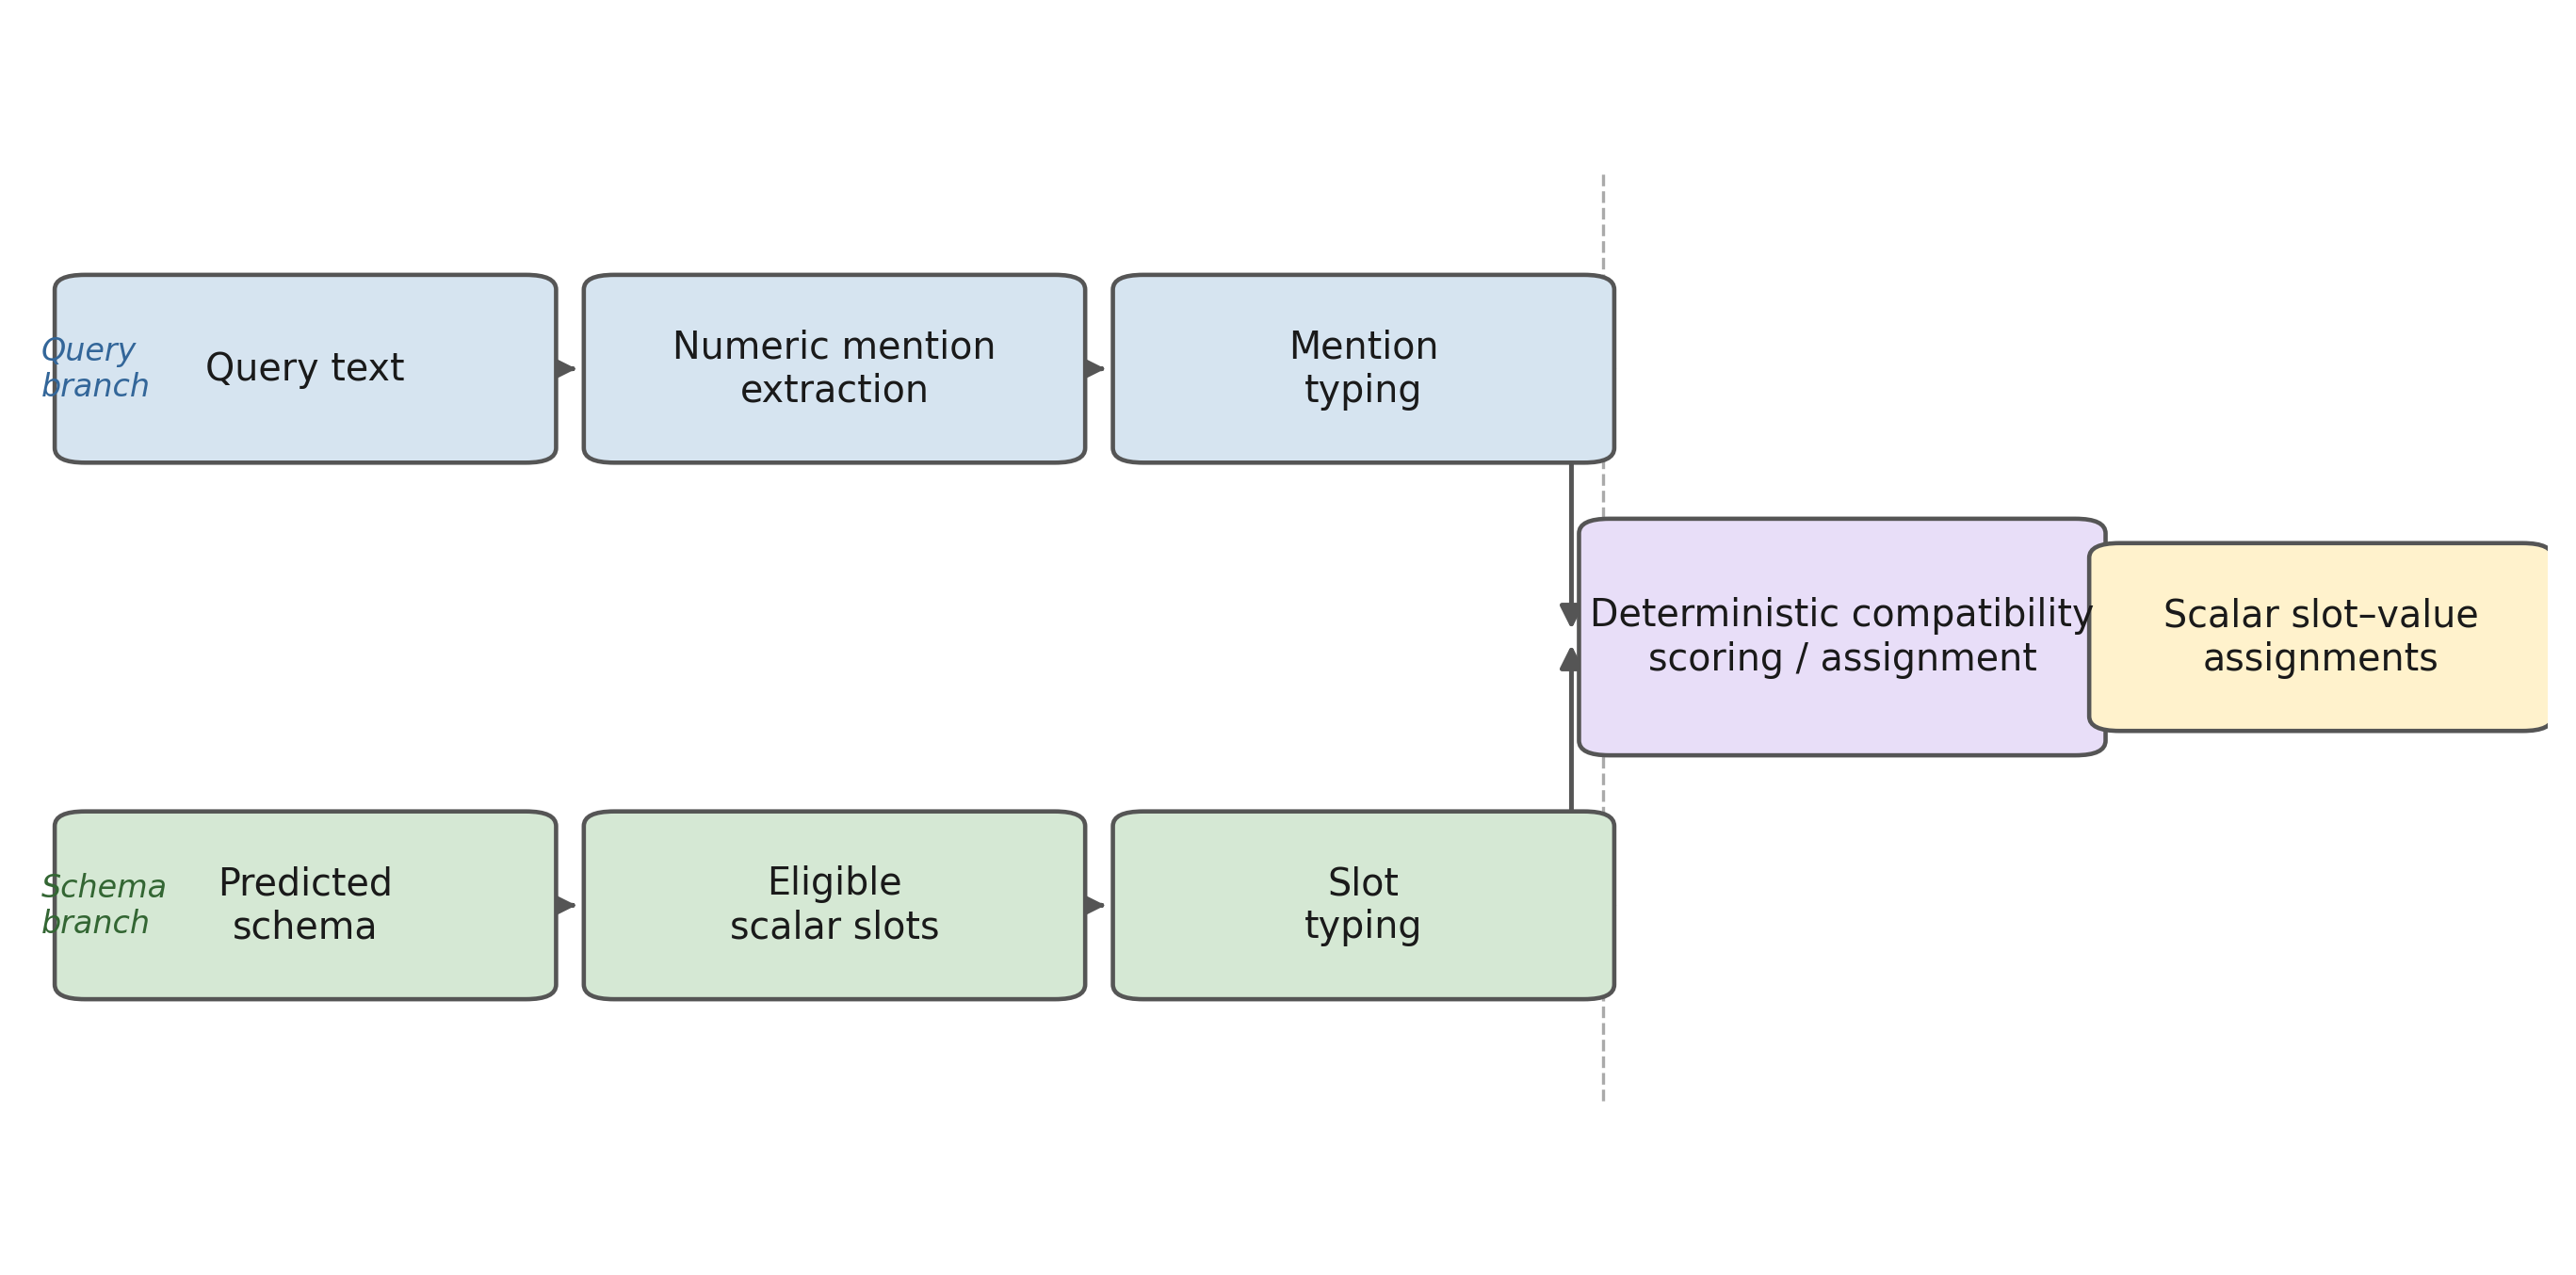
\includegraphics[width=0.82\linewidth]{figures/nlp4lp_instantiation_pipeline_v2.png}
  \caption{Schema-conditioned deterministic parameter instantiation. Numeric mentions are extracted from the query, typed using surface cues, filtered through the scalar slot inventory of the predicted schema, and assigned by a no-reuse compatibility rule. Downstream variants differ mainly in how slot--mention compatibility is scored or repaired.}
  \label{fig:instantiation-pipeline}
\end{figure}


\subsection{Evaluation-Oriented Design Choices}
\label{subsec:method_design}

The methodology is intentionally designed so that downstream evaluation remains sensitive to schema retrieval quality. In particular, the set of parameter slots eligible for instantiation is determined from the \emph{predicted} schema rather than from the gold schema. This choice is central to the formulation. If eligible slots were defined directly from the gold record, downstream coverage and readiness would no longer reflect schema-selection quality, and the evaluation would partially decouple retrieval from instantiation. By conditioning slot eligibility on the retrieved template, the framework ensures that retrieval errors propagate naturally into downstream performance through reduced structural overlap, lower slot availability, and weaker query-level readiness. At the same time, the evaluation avoids leakage: gold information is used for scoring, not for determining which schema is instantiated at inference time.

A second design choice is to restrict the main benchmarked downstream evaluation to scalar numeric parameters. This restriction is methodological rather than incidental. Scalar slots provide a common and reproducible substrate for comparing retrieval-conditioned instantiation across heterogeneous optimization templates. In contrast, list-valued and dictionary-valued parameters correspond to more structured objects, such as vectors, matrices, or indexed collections, whose recovery would require additional assumptions about alignment, dimensionality, and representation. By focusing on scalar instantiation in the core benchmark, the evaluation isolates the most comparable and interpretable component of the problem while avoiding confounding variation introduced by structured parameter reconstruction.

The use of oracle and random references serves the same interpretive purpose. The oracle condition removes retrieval error by forcing the schema prediction to equal the gold template, thereby exposing downstream behavior under perfect schema selection. This makes it possible to estimate how much room for improvement remains after retrieval. The random reference provides a lower-bound baseline: for retrieval-only evaluation, it corresponds to the theoretical top-1 chance rate under uniform schema selection, while for downstream evaluation it denotes a uniformly assigned schema passed through the same deterministic instantiation pipeline. Together, these references help separate the contribution of schema retrieval from the residual behavior of the deterministic grounding stage.

The main benchmark study is intentionally solver-free. No feasibility test, optimization run, or objective-level verification is used when computing the core retrieval and scalar-grounding metrics. This exclusion is deliberate because the main goal of the benchmark analysis is to measure the downstream utility of retrieval-assisted schema grounding and scalar parameter assignment without conflating it with formulation-completeness issues or solver-specific behavior. However, this does not mean the paper entirely ignores downstream executability. Later in the experimental section, we complement the core benchmark with engineering-oriented subset studies, including structural-validity analysis and a restricted solver-backed executable validation. These auxiliary experiments are included to assess practical downstream relevance, while the benchmark proper remains centered on schema-conditioned scalar instantiation.

The same motivation underlies the use of a fully deterministic pipeline in the core study. The benchmarked retrieval-and-grounding system does not rely on large language models, learned retrievers, \texttt{torch}-based components, or learned extractors. This design keeps the central evaluation transparent and reproducible while allowing the experiments to answer a focused question: how much structured instantiation utility can be obtained from deterministic retrieval and rule-based grounding alone? That question remains scientifically useful even when stronger downstream executability is studied separately on restricted subsets.

These design choices also determine how the reported metrics should be interpreted. In particular, \textit{InstantiationReady} should be read as a diagnostic readiness criterion based on coverage and type consistency, not as a guarantee of model correctness or solver compatibility. Likewise, strong schema retrieval should not be interpreted as full optimization-model recovery, and successful scalar assignment in the core benchmark should not be interpreted as feasibility- or optimality-verified instantiation. The restricted engineering and solver-backed subset analyses later in the paper address a different question: whether the recovered structure can support downstream executable behavior on compatible cases.

Overall, the framework is best viewed as a retrieval-assisted deterministic instantiation system whose main purpose is to quantify how schema grounding affects structured parameter recovery from natural language. This evaluation-oriented framing keeps the methodological claims aligned with the benchmark, while still leaving room for the later engineering-oriented validation studies reported in the experimental section.

\section{Experiments}
\label{sec:experiments}

\subsection{Experimental Setup}
\label{subsec:exp_setup}

We evaluate the proposed retrieval-assisted instantiation pipeline on the \textsc{NLP4LP} benchmark, which pairs natural-language optimization problem descriptions with structured optimization records and solver-oriented representations \cite{nlp4lp_dataset,ahmaditeshnizi2024optimus_icml}. Unless otherwise stated, the main benchmark results are measured on the benchmark test split, which contains 331 query instances. Each test query has exactly one gold optimization schema. In the current repository rerun, each test query is ranked against the benchmark-induced schema catalog used by the evaluation pipeline, which contains 335 candidate schema documents. Accordingly, retrieval is a 335-way top-1 identification task, and the corresponding random top-1 reference is the theoretical chance rate under uniform selection over this catalog, namely $1/335 \approx 0.0030$.

To assess robustness to surface degradation and reduced context, we evaluate three benchmark query variants. The \emph{orig} variant uses the original problem descriptions. The \emph{noisy} variant applies controlled lexical corruption, including lowercasing, token deletion, stopword reduction, and masking of some numeric expressions. The \emph{short} variant retains only the first sentence of each description. These variants allow us to test the same retrieval-and-grounding pipeline under full context, degraded wording, and substantially reduced context.

The retrieval stage ranks candidate schemas using only schema-catalog text. In the final reported benchmark comparison, we evaluate three deterministic lexical retrieval baselines: BM25 \cite{robertson2009bm25}, TF--IDF cosine retrieval implemented with \textsc{scikit-learn} \cite{pedregosa2011sklearn}, and latent semantic analysis (LSA), obtained by applying truncated singular value decomposition to TF--IDF vectors \cite{deerwester1990lsa}. In all downstream experiments, only the top-ranked schema is passed to the instantiation stage. We also report an \emph{oracle} control in which the retrieved schema is replaced by the gold schema, thereby isolating downstream grounding difficulty from retrieval error.

Given a query and a predicted schema, the downstream stage instantiates scalar parameter slots deterministically from the query text. Numeric mentions are extracted using a fixed rule-based pattern matcher. In the \emph{noisy} variant, masked numeric placeholders are preserved as special tokens but treated as numerically unknown; they may therefore still indicate the presence of a quantity without supporting exact value recovery. We restrict the core benchmarked downstream evaluation to scalar numeric parameters and exclude list-valued and dictionary-valued parameters so that the benchmark targets scalar slot grounding rather than structured arrays, matrices, or other higher-order objects.

The downstream candidate slot set is derived from the \emph{predicted} schema rather than the gold schema. When schema metadata explicitly provides parameter keys, we use those keys; otherwise, we extract keys from the predicted parameter record. These predicted keys are then intersected with scalar gold parameters to determine the subset of slots eligible for evaluation. This makes downstream evaluation intentionally retrieval-dependent: if the wrong schema is retrieved, the candidate slot inventory may already be structurally misaligned with the gold instance, which can reduce both attainable coverage and value accuracy even when the query still contains relevant numbers.

To assign extracted numbers to slots, we evaluate multiple deterministic grounding families that differ in how much structural guidance they exploit. Across all methods, scalar slots are typed using four lightweight rule-based categories: \emph{percent}, \emph{integer}, \emph{currency}, and \emph{float}. Extracted numeric mentions are mapped into the same categories using surface cues such as percentage markers, currency symbols, and integer-valued forms. The benchmark includes the original typed-greedy baselines based on TF--IDF, BM25, and LSA; an oracle typed-greedy control; and five previously reported TF--IDF-based deterministic grounding variants with additional constraints or repair mechanisms, namely constrained matching, semantic repair, optimization-role repair, acceptance reranking, and hierarchical acceptance reranking. To broaden the comparison set, we further evaluate three additional method families: \emph{global compatibility grounding}, \emph{relation-aware linking}, and \emph{ambiguity-aware grounding}. This expanded design allows us to compare simple deterministic assignment against richer structured grounding strategies while keeping the overall pipeline transparent and reproducible.

We report both retrieval effectiveness and downstream instantiation quality. \textit{Schema\_R@1} is the fraction of test queries whose top-ranked schema matches the gold schema. For downstream evaluation, let $G_i$ denote the scalar gold slots for query $i$ that are eligible for evaluation after intersecting gold scalar parameters with the candidate slots induced by the predicted schema, and let $A_i \subseteq G_i$ denote the subset of those slots that receive an assignment. Then \textit{Coverage} is
\[
\textit{Coverage}
=
\frac{\sum_i |A_i|}{\sum_i |G_i|},
\]
that is, the fraction of eligible scalar gold slots that receive any assignment. \textit{TypeMatch} is the fraction of assigned slots whose predicted numeric type matches the expected slot type,
\[
\textit{TypeMatch}
=
\frac{\sum_i |\{s \in A_i : \mathrm{type}(\hat{y}_{i,s}) = \mathrm{type}(y_{i,s})\}|}{\sum_i |A_i|},
\]
where $\hat{y}_{i,s}$ and $y_{i,s}$ denote the predicted and gold values for slot $s$ of query $i$.

To measure value accuracy, we report \textit{Exact20\_on\_hits}. This metric is computed only on the subset of \emph{schema-hit} queries for which a comparable numeric prediction and gold value are both available for the slot under consideration. A slot is counted as correct if the predicted numeric value falls within a relative error tolerance of $20\%$ of the gold value. Because meaningful numeric comparison requires both schema correctness and a comparable numeric pair, \textit{Exact20\_on\_hits} is intentionally normalized on this eligible subset rather than on all test queries. It should therefore be interpreted as a conditional value-grounding measure rather than as an end-to-end benchmark score.

Our main end-to-end utility metric is \textit{InstantiationReady}. A query is counted as \textit{InstantiationReady} if its predicted schema matches the gold schema and its instantiated scalar output satisfies the readiness rule used by our deterministic pipeline, namely: all required scalar slots that are eligible under the predicted schema receive an assignment, and each such assignment has the correct scalar type. Thus, \textit{InstantiationReady} is a strict per-instance success criterion that combines schema correctness, slot coverage, and type compatibility into a single usability-oriented diagnostic.

Unless otherwise stated, the retrieval metrics and the main downstream end-to-end metrics are reported over the full benchmark denominator for each variant. The only exception is \textit{Exact20\_on\_hits}, which is explicitly conditional on the subset of schema-hit cases with comparable numeric values. We additionally report bootstrap confidence intervals and selected paired significance analyses for key retrieval and downstream method pairs, and overlap-based stress tests -- including stratified retrieval performance by lexical-overlap level and retrieval ablations under sanitized text conditions such as number removal and stopword stripping -- to test whether strong retrieval may partly reflect benchmark-specific lexical overlap (Section~\ref{subsec:exp_significance}).

To isolate the effect of corrected numeric type handling, we also report a measured pre-fix versus post-fix ablation on four representative downstream methods across all three query variants. This ablation is especially relevant for \emph{float}-valued slots, because the corrected implementation fixes a type-handling error that had previously depressed downstream grounding quality. Both the post-fix benchmark and the pre/post ablation are measured on the canonical \textsc{NLP4LP} test benchmark.

Finally, to complement the core benchmark with downstream practical evidence, we include three engineering-oriented validation studies (Section~\ref{subsec:exp_engineering}): (i) a structural engineering subset experiment, (ii) an executable-attempt study on the largest deterministic executable-eligible subset available in the local cache, and (iii) a restricted solver-backed final-attempt study on a small compatibility-filtered subset. These auxiliary studies are not replacements for the main benchmark; rather, they assess whether the recovered structure can support increasingly concrete downstream optimization behavior on restricted subsets. Table~\ref{tab:exp_blocks} summarizes the overall experimental design.

All experiments are deterministic and primarily CPU-based. The implementation uses standard data-processing and retrieval libraries, including Hugging Face \texttt{datasets} \cite{lhoest2021datasets} and \textsc{scikit-learn} \cite{pedregosa2011sklearn}. The core benchmarked evaluation uses no large language model prompting, no custom neural training procedure, and no solver-based scoring. This setup is deliberate: it isolates the contribution of schema retrieval and deterministic number-to-slot grounding while keeping the central evaluation procedure transparent and reproducible.

\begin{table}[t]
\centering
\caption{Summary of the experimental blocks used in the paper.}
\label{tab:exp_blocks}
\scriptsize
\begin{tabularx}{\linewidth}{l l X}
\hline
Block & Primary purpose & Main outputs \\
\hline
Main benchmark & Retrieval and scalar grounding on \textsc{NLP4LP} & Schema\_R@1, Coverage, TypeMatch, Exact20\_on\_hits, InstantiationReady \\
Robustness analyses & Sensitivity to degraded input and lexical overlap & Orig / noisy / short comparisons, overlap-based stress tests \\
Pre/post ablation & Isolate effect of corrected type handling & TypeMatch and InstantiationReady changes \\
Significance testing & Assess whether reported gaps are statistically robust & Paired bootstrap $p$-values and confidence intervals \\
Engineering subset validation (60 inst.) & Assess downstream structural usefulness & Structural-validity and instantiation-completeness rates \\
Executable-attempt subset (269 inst.) & Document restricted downstream executability and blockers & Executable, solver-success, feasibility, and objective-produced rates \\
Final solver-backed subset (20 inst.) & Real, restricted solver execution via SciPy HiGHS shim & Executable, solver-success, feasible, and objective-produced rates \\
\hline
\end{tabularx}
\end{table}

\subsection{Schema Retrieval Performance}
\label{subsec:exp_retrieval}

We first evaluate schema retrieval in isolation to determine whether selecting the correct benchmark schema is itself a major source of error in the present fixed-catalog setting. Table~\ref{tab:nlp4lp-retrieval-main} reports \textit{Schema\_R@1}, defined as the fraction of test queries for which the top-ranked retrieved schema matches the gold schema, across the three query variants described in Section~\ref{subsec:exp_setup}. In the current repository rerun, retrieval is evaluated against the benchmark catalog stored in \texttt{data/catalogs/nlp4lp\_catalog.jsonl}, which contains 335 candidate schema documents. Accordingly, the random reference corresponds to the theoretical top-1 chance rate under uniform selection over this catalog, namely $1/335 \approx 0.0030$.

The purpose of this experiment is deliberately limited. We do not treat it as an open-domain optimization retrieval task or as evidence that lexical retrieval alone would suffice in broader real-world schema libraries. Rather, within the benchmark-induced candidate set, we ask whether simple deterministic retrieval can identify the single schema document that provides the downstream scalar slot inventory used by the grounding stage. This benchmark-scoped retrieval analysis is therefore intended to characterize the structural conditions under which downstream instantiation operates, not to claim a general solution to schema retrieval in unrestricted optimization-modeling environments.

Within this fixed-catalog benchmark, lexical schema retrieval is already strong. On the original queries, TF--IDF achieves the best performance with \textit{Schema\_R@1} $= 0.9094$, followed by BM25 at $0.8822$ and LSA at $0.8459$. All three methods are far above the random baseline, indicating that the benchmark descriptions contain enough schema-level textual evidence for recovering the correct benchmark template in most cases. Thus, in the canonical test setting studied here, schema identification is substantially easier than the downstream instantiation problem studied later in the paper.

Retrieval also remains strong under controlled lexical degradation. On the \emph{noisy} queries, TF--IDF, BM25, and LSA achieve \textit{Schema\_R@1} values of $0.9033$, $0.8912$, and $0.8882$, respectively. These values are close to their corresponding results on the original queries. This stability suggests that benchmark-level schema identification is not highly sensitive to moderate perturbations such as lowercasing, token deletion, stopword reduction, and numeric masking, even though the retrieval backbones themselves remain lexical rather than semantics-aware.

The \emph{short} setting is more challenging. When each description is truncated to its first sentence, \textit{Schema\_R@1} decreases to $0.7795$ for TF--IDF, $0.7674$ for BM25, and $0.7644$ for LSA. This drop is expected because truncation removes contextual details that often distinguish closely related benchmark formulations. Even so, performance remains well above chance for all three methods, showing that substantial benchmark-specific schema evidence is often present in the opening sentence alone.

Across all three variants, TF--IDF again achieves the best average retrieval accuracy ($0.8641$), with BM25 close behind ($0.8469$) and LSA somewhat lower but still competitive ($0.8328$). We therefore use TF--IDF as the main retrieval backbone in the downstream experiments. More importantly, the absolute retrieval levels in Table~\ref{tab:nlp4lp-retrieval-main} establish the main benchmark-level interpretive point for the remainder of the paper: within this fixed-catalog \textsc{NLP4LP} setting, the dominant limitation is not selecting a plausible schema document, but grounding the numerical content of the query to the appropriate scalar roles once such a schema has been selected. This conclusion is intentionally benchmark-scoped and should not be read as a claim that schema retrieval is solved in broader optimization-modeling settings.

\begin{table}[t]
  \centering
  \caption{Schema retrieval accuracy across query variants, reported as \textit{Schema\_R@1}. Each value is computed over all 331 test queries in the corresponding variant. The random baseline is the theoretical top-1 chance rate under uniform schema selection over the 335 candidate schemas used in the current repository rerun, i.e., $1/335 \approx 0.0030$. Best result in each column is shown in bold.}
  \label{tab:nlp4lp-retrieval-main}
  \small
  \setlength{\tabcolsep}{4pt}
  \resizebox{\linewidth}{!}{%
  \begin{tabular}{lcccc}
    \hline
    Baseline & Orig & Noisy & Short & Avg. \\
    \hline
    Random  & 0.0030 & 0.0030 & 0.0030 & 0.0030 \\
    LSA     & 0.8459 & 0.8882 & 0.7644 & 0.8328 \\
    BM25    & 0.8822 & 0.8912 & 0.7674 & 0.8469 \\
    TF--IDF & \textbf{0.9094} & \textbf{0.9033} & \textbf{0.7795} & \textbf{0.8641} \\
    \hline
  \end{tabular}%
  }
\end{table}


\subsection{Downstream Utility for Problem Instantiation}
\label{subsec:exp_downstream}

We next evaluate whether correct or near-correct schema retrieval translates into useful downstream instantiation within the restricted scalar-grounding setting studied in this paper. In the proposed pipeline, the retrieved schema determines the candidate scalar slot inventory, after which deterministic numeric extraction and slot assignment are applied as described in Section~\ref{subsec:exp_setup}. The central question is not whether the system can recover a complete optimization model, but whether successful schema selection yields scalar slot--value assignments that are sufficiently complete and type-consistent to provide measurable intermediate support for optimization modeling.

Table~\ref{tab:nlp4lp-downstream-main} reports the main post-fix downstream results on the \emph{orig} queries for the original deterministic grounding family. Three findings are most important. First, deterministic retrieval-assisted grounding recovers a substantial amount of scalar structure on the original benchmark inputs. Under the strongest non-oracle setting among the original methods, \texttt{tfidf\_typed\_greedy} reaches \textit{Coverage} $=0.8639$, \textit{TypeMatch} $=0.7513$, and \textit{InstantiationReady} $=0.5257$. The corresponding BM25 and LSA typed-greedy variants remain close, with \textit{InstantiationReady} values of $0.5196$ and $0.4985$, respectively. Within this benchmarked scalar task, these results show that a deterministic retrieval-assisted pipeline can recover a large fraction of eligible scalar assignments with the correct coarse type.

Second, the best conditional value-accuracy score does not coincide with the best end-to-end utility. \texttt{tfidf\_constrained} achieves the strongest \textit{Exact20\_on\_hits} score ($0.3293$), and \texttt{tfidf\_semantic\_ir\_repair} achieves the strongest non-oracle \textit{TypeMatch} score ($0.7549$), but neither yields the best \textit{InstantiationReady}. As defined in Section~\ref{subsec:exp_setup}, \textit{Exact20\_on\_hits} is a conditional metric computed only on eligible schema-hit cases with comparable numeric values, whereas \textit{InstantiationReady} is a strict full-denominator query-level criterion. The results therefore show that local gains on a restricted comparable subset do not automatically translate into stronger query-level readiness. In this benchmark, downstream usefulness depends on balancing coverage, type compatibility, and retrieval-conditioned structural fit rather than maximizing a single local matching score.

Third, the oracle control confirms that retrieval matters but is not the dominant remaining source of error within this benchmark. Replacing \texttt{tfidf\_typed\_greedy} with \texttt{oracle\_typed\_greedy} increases \textit{Coverage} from $0.8639$ to $0.9151$, \textit{TypeMatch} from $0.7513$ to $0.8030$, and \textit{InstantiationReady} from $0.5257$ to $0.5650$. These gains are meaningful but still modest relative to the remaining gap to perfect instantiation. Even when the correct schema is supplied, substantial difficulty remains in deciding which extracted quantity should fill which scalar slot. This is the central benchmark-level empirical point of the paper: on \textsc{NLP4LP}, schema retrieval is already comparatively strong, whereas downstream number-to-slot grounding remains the main unresolved source of error.

To test whether richer deterministic grounding can materially improve this stage, we added three new downstream method families in the repository rerun: global compatibility grounding (GCG), relation-aware linking (RAL), and ambiguity-aware grounding (AAG). In total, these additions produced 33 new result files covering 11 new method variants across the three query forms. The most important outcome is negative but informative: none of the newly added downstream families surpasses the simple \texttt{tfidf\_typed\_greedy} baseline on the original benchmark. Table~\ref{tab:nlp4lp-downstream-newfamilies} summarizes representative results. The best new representative, \texttt{tfidf\_relation\_aware\_basic}, reaches \textit{InstantiationReady} $=0.4985$, still below the typed-greedy baseline. The strongest tested global-compatibility and ambiguity-aware representatives, \texttt{tfidf\_global\_compat\_full} and \texttt{tfidf\_ambiguity\_aware\_beam}, perform substantially worse at $0.4320$ and $0.4230$, respectively, while the abstention-heavy ambiguity variant becomes overly conservative ($0.0272$). These reruns therefore strengthen the paper's main conclusion: the bottleneck is not merely the absence of additional deterministic structure or more careful search. Rather, the underlying quantity-to-role grounding problem remains difficult even after adding richer assignment families.

A related observation is that several of the strongest original non-oracle methods perform very similarly on \emph{orig}. The gap among TFIDF-TG ($0.5257$), TFIDF-AR ($0.5227$), BM25-TG ($0.5196$), and TFIDF-HAR ($0.5136$) is small. The new rerun results do not change this picture. Instead, they suggest that once schema retrieval is already strong, incremental changes to local assignment, compatibility scoring, beam search, or conservative abstention produce only limited gains unless they resolve the deeper semantic ambiguity of quantity-to-role matching. Put differently, the main downstream opportunity is not simply choosing among nearby deterministic search strategies, but improving how extracted numbers are semantically anchored to the correct parameter roles.

Table~\ref{tab:nlp4lp-downstream-variants} summarizes representative methods across the three query variants. The cross-variant comparison helps separate two different failure modes. In the \emph{noisy} variant, retrieval remains fairly strong, but downstream readiness collapses because many numeric values are intentionally masked; exact value recovery is therefore structurally underdetermined. This is reflected in very low \textit{InstantiationReady} values across all methods, including the oracle control. In the \emph{short} variant, the main issue is not masking but missing context: the first sentence often does not contain enough quantitative or semantic evidence to support broad slot filling. Here the main bottleneck becomes low \textit{Coverage}. Among the representative original methods, \texttt{tfidf\_acceptance\_rerank} achieves the strongest \textit{InstantiationReady} on \emph{short} ($0.0211$), but the absolute values remain very low, indicating that aggressive truncation removes much of the information needed for reliable scalar grounding.

Taken together, these results support a narrower but more defensible interpretation of system utility. On original benchmark inputs, deterministic retrieval-assisted grounding can produce partially usable scalar instantiations for a substantial fraction of cases, and the strongest measured non-oracle method remains \texttt{tfidf\_typed\_greedy} at $0.5257$ \textit{InstantiationReady} on the 331-query test split. At the same time, the updated comparison set shows that adding richer deterministic downstream structure does not by itself close the remaining gap, while the oracle ceiling remains only $0.5650$. The framework should therefore be interpreted as a transparent retrieval-and-grounding component for optimization problem instantiation on a fixed benchmark, not as a complete natural-language-to-optimization automation system. The downstream results are meaningful precisely as benchmarked evidence about this restricted intermediate task, not as a claim of full semantic understanding or broad real-world optimization-model recovery.

\begin{table}[t]
  \centering
  \caption{Main post-fix downstream results on the \emph{orig} queries for the original deterministic grounding family. \textit{Coverage}, \textit{TypeMatch}, and \textit{InstantiationReady} use the full 331-query denominator. \textit{Exact20\_on\_hits} is conditional on eligible schema-hit cases with comparable numeric values. Best non-oracle result in each column is bold.}
  \label{tab:nlp4lp-downstream-main}
  \scriptsize
  \setlength{\tabcolsep}{3.8pt}
  \begin{tabular}{lcccc}
    \hline
    Method & Coverage & TypeMatch & Exact20 & InstReady \\
    \hline
    TFIDF-TG  & \textbf{0.8639} & 0.7513 & 0.1991 & \textbf{0.5257} \\
    BM25-TG   & 0.8509 & 0.7386 & 0.2057 & 0.5196 \\
    LSA-TG    & 0.8176 & 0.7028 & 0.2048 & 0.4985 \\
    Oracle-TG & 0.9151 & 0.8030 & 0.1882 & 0.5650 \\
    TFIDF-CON & 0.8112 & 0.7113 & \textbf{0.3293} & 0.4230 \\
    TFIDF-SIR & 0.7817 & \textbf{0.7549} & 0.2843 & 0.4864 \\
    TFIDF-ORR & 0.8248 & 0.7036 & 0.2847 & 0.4411 \\
    TFIDF-AR  & 0.8332 & 0.7340 & 0.1994 & 0.5227 \\
    TFIDF-HAR & 0.8121 & 0.7146 & 0.2003 & 0.5136 \\
    \hline
  \end{tabular}

  \vspace{2mm}
  \raggedright
  \footnotesize
  Abbreviations: TFIDF-TG = \texttt{tfidf\_typed\_greedy}, BM25-TG = \texttt{bm25\_typed\_greedy}, LSA-TG = \texttt{lsa\_typed\_greedy}, Oracle-TG = \texttt{oracle\_typed\_greedy}, TFIDF-CON = \texttt{tfidf\_constrained}, TFIDF-SIR = \texttt{tfidf\_semantic\_ir\_repair}, TFIDF-ORR = \texttt{tfidf\_optimization\_role\_repair}, TFIDF-AR = \texttt{tfidf\_acceptance\_rerank}, and TFIDF-HAR = \texttt{tfidf\_hierarchical\_acceptance\_rerank}.
\end{table}

\begin{table}[t]
  \centering
  \caption{Representative \emph{orig}-query \textit{InstantiationReady} results for the newly added downstream families. None of the new deterministic grounding families surpasses the original \texttt{tfidf\_typed\_greedy} baseline.}
  \label{tab:nlp4lp-downstream-newfamilies}
  \scriptsize
  \setlength{\tabcolsep}{4pt}
  \begin{tabular}{lc}
    \hline
    Method & InstReady \\
    \hline
    TFIDF-TG                      & \textbf{0.5257} \\
    TFIDF-AR                      & 0.5227 \\
    Oracle-TG                     & 0.5650 \\
    RAL-Basic                     & 0.4985 \\
    GCG-Full                      & 0.4320 \\
    AAG-Beam                      & 0.4230 \\
    AAG-Abstain                   & 0.0272 \\
    \hline
  \end{tabular}

  \vspace{2mm}
  \raggedright
  \footnotesize
  Abbreviations: GCG-Full = \texttt{tfidf\_global\_compat\_full}, RAL-Basic = \texttt{tfidf\_relation\_aware\_basic}, and AAG-Beam/AAG-Abstain = \texttt{tfidf\_ambiguity\_aware\_beam}/\texttt{tfidf\_ambiguity\_aware\_abstain}.
\end{table}

\begin{table}[t]
  \centering
  \caption{Cross-variant downstream summary for representative original methods. The \emph{noisy} variant should be interpreted cautiously because masked numeric values make exact grounding structurally difficult even when the schema is correct.}
  \label{tab:nlp4lp-downstream-variants}
  \scriptsize
  \setlength{\tabcolsep}{3.2pt}
  \begin{tabular}{lcccccc}
    \hline
    Method & O-Cov & N-Cov & S-Cov & O-IR & N-IR & S-IR \\
    \hline
    TFIDF-TG  & 0.8639 & 0.7693 & 0.1050 & 0.5257 & 0.0393 & 0.0151 \\
    BM25-TG   & 0.8509 & 0.7620 & 0.1062 & 0.5196 & 0.0423 & 0.0151 \\
    TFIDF-AR  & 0.8332 & 0.7312 & 0.1130 & 0.5227 & 0.0423 & \textbf{0.0211} \\
    Oracle-TG & 0.9151 & 0.8196 & 0.1258 & \textbf{0.5650} & 0.0423 & 0.0151 \\
    \hline
  \end{tabular}

  \vspace{2mm}
  \raggedright
  \footnotesize
  O = \emph{orig}, N = \emph{noisy}, S = \emph{short}, and IR = \textit{InstantiationReady}.
\end{table}

\subsection{Error Analysis and Ablation Studies}
\label{subsec:exp_error}

To better understand the remaining gap between strong schema retrieval and reliable downstream instantiation, we examine three complementary diagnostics derived from the measured repository artifacts: a diagnostic error taxonomy from the final post-fix benchmark, a pre-fix versus post-fix ablation of the corrected numeric type-handling logic, and a comparison against the newly added downstream method families. Together, these analyses clarify where the deterministic pipeline still fails and why the final post-fix benchmark should be interpreted as materially more reliable than the earlier intermediate-development results.

A first point is that the dominant residual errors arise primarily \emph{after} schema retrieval rather than \emph{at} schema retrieval. As shown in Section~\ref{subsec:exp_retrieval}, TF--IDF retrieves the correct schema for $0.9094$ of the \emph{orig} test queries, leaving limited room for large gains from retrieval alone. The diagnostic breakdown in Table~\ref{tab:nlp4lp-error-taxonomy} is consistent with this interpretation. Although wrong-schema retrieval remains a real source of failure, larger diagnostic counts are associated with downstream grounding effects, especially type mismatches, role confusion among semantically related quantities, and wrong-slot disambiguation. Thus, once the structural template is approximately correct, the main difficulty becomes deciding which extracted number should populate which scalar role.

Among these downstream phenomena, type-related failures are especially influential. In the benchmark, many scalar values are not explicitly marked as percentages or currency amounts and are not naturally restricted to integer form. These more weakly marked continuous quantities are therefore more vulnerable to type-handling and compatibility errors than clearly signaled surface forms. Before correction, such cases disproportionately suppressed both \textit{TypeMatch} and query-level \textit{InstantiationReady}. This matters substantively, not merely implementation-wise: type compatibility is one of the gates through which a plausible extracted quantity becomes a usable slot filling. The corrected benchmark therefore changes the interpretation of the system. The pipeline is no longer best described as failing mainly because it cannot identify the right schema; rather, it identifies the schema correctly in most cases and then encounters its main remaining difficulty in semantically grounded number-to-slot assignment.

The error taxonomy should be interpreted as diagnostic rather than as a disjoint exhaustive partition. The categories in Table~\ref{tab:nlp4lp-error-taxonomy} are approximate counts derived from the final measured benchmark and associated diagnostic reports, and a single query may contribute to more than one category. We use them to identify the main error families, not to claim a formal one-label decomposition of all failures. Even with that caution, the pattern is clear: the largest counts are downstream and semantics-related, whereas unsupported schemas are absent and pure extraction misses are comparatively rare. This strengthens the paper's main empirical claim that the remaining bottleneck lies in grounding rather than in retrieval.

Table~\ref{tab:nlp4lp-prefix-postfix} quantifies the effect of the corrected type-handling logic. On the \emph{orig} queries, the post-fix version improves \textit{TypeMatch} by $0.4918$ for TFIDF-TG, $0.4320$ for TFIDF-ORR, $0.4553$ for TFIDF-HAR, and $0.5145$ for Oracle-TG. These are large changes, and they produce correspondingly large gains in \textit{InstantiationReady}. For example, TFIDF-TG rises from $0.0695$ to $0.5257$, and Oracle-TG rises from $0.0785$ to $0.5650$. By contrast, extraction-dependent quantities change much less. This is exactly what one would expect from the nature of the correction: the system is largely extracting similar candidate numbers, but it is now handling value-type compatibility with the target slot much more accurately.

The repository rerun also provides a stronger test of whether richer downstream structure can resolve the remaining errors. We added three new deterministic method families---global compatibility grounding (GCG), relation-aware linking (RAL), and ambiguity-aware grounding (AAG)---and reran all 11 new variants across the three benchmark query forms. The most informative result is that these additions do \emph{not} overturn the original bottleneck diagnosis. As summarized in Table~\ref{tab:nlp4lp-newfamily-errorcheck}, none of the strongest new representatives surpasses the original \texttt{tfidf\_typed\_greedy} baseline on \emph{orig}. The best new representative, \texttt{tfidf\_relation\_aware\_basic}, reaches \textit{InstantiationReady} $=0.4985$, still below TFIDF-TG ($0.5257$). The strongest tested global-compatibility and ambiguity-aware representatives, \texttt{tfidf\_global\_compat\_full} and \texttt{tfidf\_ambiguity\_aware\_beam}, fall further to $0.4320$ and $0.4230$, respectively, and the abstention-heavy ambiguity variant becomes overly conservative ($0.0272$). Thus, even after adding more structured local linking, slot--slot compatibility terms, beam-style search, and explicit ambiguity handling, the remaining grounding errors are not easily removed.

This negative result is important because it shows that the residual gap is not simply due to a lack of downstream engineering variety. Rather, the unresolved failures reflect genuinely difficult semantic ambiguities: totals versus unit coefficients, lower versus upper bounds, percentages versus absolute values, and generic continuous values whose local lexical context is weak. The rerun therefore strengthens the main interpretation of the benchmark. Once retrieval is already strong, adding richer deterministic search or compatibility machinery does not by itself close the gap to robust query-level readiness.

The pre/post comparison is also useful for interpreting the robustness patterns from Section~\ref{subsec:exp_downstream}. In the \emph{noisy} variant, the post-fix gains are real but much smaller. For TFIDF-TG, \textit{TypeMatch} increases from $0.0583$ to $0.1414$, while \textit{InstantiationReady} rises only from $0.0211$ to $0.0393$. This does not indicate that the correction was unimportant; rather, it reflects the structure of the benchmark variant itself. When numeric values are intentionally masked, downstream grounding becomes underdetermined even if the schema is correct. In the \emph{short} variant, the correction again helps, but readiness remains very low because the first sentence often lacks enough contextual and numeric evidence for broad slot filling. The corrected post-fix benchmark therefore resolves a major compatibility problem on the original inputs while also showing that downstream performance still depends strongly on the availability of explicit quantitative evidence.

Overall, the error analysis and ablation studies reinforce the central conclusion of the paper. On \textsc{NLP4LP}, the main bottleneck is not schema retrieval; it is number-to-slot grounding under semantic ambiguity. The corrected post-fix benchmark provides a substantially stronger empirical basis for evaluating this stage, and the expanded rerun shows that even richer deterministic grounding families do not materially surpass the simple TF--IDF typed-greedy baseline. Future improvements should therefore focus less on incremental deterministic search refinements and more on substantially stronger semantic grounding of quantities to parameter roles.

\begin{table}[t]
  \centering
  \caption{Diagnostic error taxonomy for TF--IDF on the \emph{orig} queries. Counts are approximate diagnostic indicators derived from the final measured benchmark and associated reports; categories are not disjoint, and a single query may contribute to multiple categories.}
  \label{tab:nlp4lp-error-taxonomy}
  \small
  \setlength{\tabcolsep}{4pt}
  \begin{tabular}{p{4.7cm}c}
    \hline
    Error type & Count \\
    \hline
    Wrong schema retrieval & $\approx 30$ \\
    Missing numeric extraction & 5 \\
    Wrong type assignment (mainly float-related) & 230 \\
    Wrong slot disambiguation & 50 \\
    Total vs.\ unit confusion & 20 \\
    Min/max inversion & 10 \\
    Percent vs.\ absolute confusion & 15 \\
    Float ambiguity with many candidate values & 25 \\
    Unsupported schema & 0 \\
    \hline
  \end{tabular}
\end{table}

\begin{table}[t]
  \centering
  \caption{Measured pre-fix versus post-fix ablation on four representative methods across the three query variants. The correction mainly affects \textit{TypeMatch} and \textit{InstantiationReady}, while leaving extraction-dependent quantities much less changed.}
  \label{tab:nlp4lp-prefix-postfix}
  \scriptsize
  \setlength{\tabcolsep}{3.2pt}
  \begin{tabular}{llcccccc}
    \hline
    Var. & Method & Type$_{\text{pre}}$ & Type$_{\text{post}}$ & $\Delta$Type & IR$_{\text{pre}}$ & IR$_{\text{post}}$ & $\Delta$IR \\
    \hline
    orig  & TFIDF-TG  & 0.2595 & 0.7513 & 0.4918 & 0.0695 & 0.5257 & 0.4562 \\
    orig  & TFIDF-ORR & 0.2716 & 0.7036 & 0.4320 & 0.0665 & 0.4411 & 0.3746 \\
    orig  & TFIDF-HAR & 0.2593 & 0.7146 & 0.4553 & 0.0785 & 0.5136 & 0.4351 \\
    orig  & Oracle-TG & 0.2885 & 0.8030 & 0.5145 & 0.0785 & 0.5650 & 0.4865 \\
    \hline
    noisy & TFIDF-TG  & 0.0583 & 0.1414 & 0.0831 & 0.0211 & 0.0393 & 0.0182 \\
    noisy & TFIDF-ORR & 0.0000 & 0.0000 & 0.0000 & 0.0000 & 0.0000 & 0.0000 \\
    noisy & TFIDF-HAR & 0.0647 & 0.1380 & 0.0733 & 0.0242 & 0.0423 & 0.0181 \\
    noisy & Oracle-TG & 0.0703 & 0.1524 & 0.0821 & 0.0211 & 0.0423 & 0.0212 \\
    \hline
    short & TFIDF-TG  & 0.0962 & 0.2286 & 0.1324 & 0.0060 & 0.0151 & 0.0091 \\
    short & TFIDF-ORR & 0.0438 & 0.0725 & 0.0287 & 0.0060 & 0.0060 & 0.0000 \\
    short & TFIDF-HAR & 0.1133 & 0.2261 & 0.1128 & 0.0091 & 0.0211 & 0.0120 \\
    short & Oracle-TG & 0.1133 & 0.2709 & 0.1576 & 0.0030 & 0.0151 & 0.0121 \\
    \hline
  \end{tabular}

  \vspace{2mm}
  \raggedright
  \footnotesize
  Abbreviations: IR = \textit{InstantiationReady}, TFIDF-TG = \texttt{tfidf\_typed\_greedy}, TFIDF-ORR = \texttt{tfidf\_optimization\_role\_repair}, TFIDF-HAR = \texttt{tfidf\_hierarchical\_acceptance\_rerank}, and Oracle-TG = \texttt{oracle\_typed\_greedy}.
\end{table}

\begin{table}[t]
  \centering
  \caption{Representative \emph{orig}-query \textit{InstantiationReady} comparison between the original TF--IDF baseline, the oracle reference, and the strongest representatives of the three newly added downstream families. Reported deltas are relative to TFIDF-TG.}
  \label{tab:nlp4lp-newfamily-errorcheck}
  \small
  \setlength{\tabcolsep}{4pt}
  \begin{tabular}{lccc}
    \hline
    Method & InstReady & $\Delta$ vs.\ TFIDF-TG & Note \\
    \hline
    TFIDF-TG    & 0.5257 & 0.0000  & baseline \\
    TFIDF-AR    & 0.5227 & -0.0030 & near tie \\
    RAL-Basic   & 0.4985 & -0.0272 & below baseline \\
    GCG-Full    & 0.4320 & -0.0937 & markedly lower \\
    AAG-Beam    & 0.4230 & -0.1027 & markedly lower \\
    AAG-Abstain & 0.0272 & -0.4985 & overly conservative \\
    Oracle-TG   & 0.5650 & +0.0393 & upper reference \\
    \hline
  \end{tabular}

  \vspace{2mm}
  \raggedright
  \footnotesize
  Abbreviations: GCG-Full = \texttt{tfidf\_global\_compat\_full}, RAL-Basic = \texttt{tfidf\_relation\_aware\_basic}, AAG-Beam = \texttt{tfidf\_ambiguity\_aware\_beam}, and AAG-Abstain = \texttt{tfidf\_ambiguity\_aware\_abstain}.
\end{table}

\subsection{Statistical Significance and Lexical-Overlap Robustness}
\label{subsec:exp_significance}

Section~\ref{subsec:exp_setup} noted that key retrieval and downstream comparisons are supported by paired bootstrap significance tests and by overlap-based stress tests; we report both here.

Using a paired bootstrap with $B=1{,}000$ resamples over the 331 \emph{orig} test queries, the \textit{InstantiationReady} gap between TF--IDF and Oracle is statistically significant ($\Delta=-0.0393$, 95\% CI $[-0.0665,-0.0151]$, $p=0.004$), confirming that the modest oracle improvement discussed in Section~\ref{subsec:exp_downstream} is unlikely to be a sampling artifact. The \textit{Schema\_R@1} gap between TF--IDF and BM25 is only marginally significant ($\Delta=+0.0272$, $p=0.022$). TF--IDF typed-greedy is statistically indistinguishable from the acceptance-rerank and hierarchical-acceptance-rerank variants ($p=0.890$ and $p=0.376$), but significantly outperforms representative global-compatibility, relation-aware, and ambiguity-aware variants on \textit{InstantiationReady} ($p<0.001$ in the tested comparisons; Table~\ref{tab:nlp4lp-significance}). This confirms that the negative result for the newly added method families in Section~\ref{subsec:exp_downstream} is not an artifact of sampling noise.

To test whether strong lexical retrieval mainly reflects benchmark-specific numeric overlap between query and schema text, we re-ran TF--IDF, BM25, and LSA retrieval after stripping numeric tokens and/or stopwords from the query. Table~\ref{tab:nlp4lp-overlap} shows that TF--IDF and BM25 accuracy is stable or slightly \emph{higher} once numbers and stopwords are removed, indicating that retrieval success is driven by structural and domain-term overlap (parameter names, units, problem-type keywords) rather than by matching the specific numeric values in the query. The baseline row in Table~\ref{tab:nlp4lp-overlap} comes from a separate diagnostic rerun of the retrieval harness and differs slightly from the canonical value in Table~\ref{tab:nlp4lp-retrieval-main} ($0.9063$ vs.\ $0.9094$ for TF--IDF) due to minor preprocessing differences between the two evaluation scripts; both values support the same qualitative conclusion, and we report the discrepancy rather than silently reconciling it. A complementary stratification by query--schema lexical (Jaccard) overlap shows most \emph{orig} queries (327 of 331) fall in a high-overlap bucket with TF--IDF \textit{Schema\_R@1} $=0.9205$; the remaining low-overlap bucket has only 4 queries and is too small to support a separate quantitative claim, so we report it only as a qualitative caveat on the generality of the overlap analysis.

\begin{table}[t]
\centering
\caption{Paired bootstrap significance tests ($B=1{,}000$ resamples, \emph{orig} queries) for selected retrieval and downstream comparisons. Diff is method A minus method B on the stated metric.}
\label{tab:nlp4lp-significance}
\scriptsize
\setlength{\tabcolsep}{4pt}
\begin{tabular}{lccc}
  \hline
  Comparison (metric) & Diff & 95\% CI & $p$ \\
  \hline
  TFIDF vs.\ BM25 (Schema\_R@1) & +0.0272 & [+0.0060, +0.0514] & 0.022 \\
  TFIDF-TG vs.\ Oracle-TG (InstReady) & -0.0393 & [-0.0665, -0.0151] & 0.004 \\
  TFIDF-TG vs.\ TFIDF-AR (InstReady) & +0.0030 & [-0.0181, +0.0211] & 0.890 \\
  TFIDF-TG vs.\ TFIDF-HAR (InstReady) & +0.0121 & [-0.0121, +0.0363] & 0.376 \\
  TFIDF-TG vs.\ GCG-Full (InstReady) & +0.0937 & [+0.0483, +0.1420] & $<0.001$ \\
  TFIDF-TG vs.\ RAL-Basic (InstReady) & +0.0272 & [-0.0091, +0.0665] & 0.218 \\
  TFIDF-TG vs.\ AAG-Beam (InstReady) & +0.1027 & [+0.0514, +0.1511] & $<0.001$ \\
  \hline
\end{tabular}
\end{table}

\begin{table}[t]
\centering
\caption{Retrieval accuracy (\textit{Schema\_R@1}, \emph{orig} queries) after removing numeric tokens and/or stopwords, from a separate diagnostic rerun of the retrieval harness (hence the small offset from Table~\ref{tab:nlp4lp-retrieval-main}).}
\label{tab:nlp4lp-overlap}
\small
\begin{tabular}{lccc}
  \hline
  Sanitization & TF--IDF & BM25 & LSA \\
  \hline
  None (baseline)               & 0.9063 & 0.8852 & 0.7734 \\
  Numbers removed               & 0.9063 & 0.8973 & 0.7734 \\
  Stopwords removed             & 0.9124 & 0.9063 & 0.8731 \\
  Numbers \& stopwords removed  & 0.9124 & 0.9063 & 0.8731 \\
  \hline
\end{tabular}
\end{table}

\subsection{Engineering-Oriented and Solver-Backed Validation}
\label{subsec:exp_engineering}

The benchmark above is deliberately solver-free: no feasibility test or objective evaluation enters \textit{Schema\_R@1}, \textit{Coverage}, \textit{TypeMatch}, or \textit{InstantiationReady}. To assess whether the recovered schema-conditioned structure has any downstream executable value, we report three restricted engineering-oriented validation studies on subsets of \textsc{NLP4LP} for which the gold record contains executable solver code (\texttt{optimus\_code}). These studies use the SciPy HiGHS mixed-integer-linear-programming solver through a compatibility shim; \emph{Gurobi is not required} to reproduce any of the results below. All three studies are restricted in scope by construction and are not claims of benchmark-wide executability.

\paragraph{Structural engineering subset (60 instances).} Table~\ref{tab:eng-structural} and Figure~\ref{fig:eng-validation} report schema-hit rate, structural-validity rate (LP objective/variable consistency checked without a live solver), and instantiation-completeness rate on a 60-instance engineering-flavored subset. TF--IDF reaches a structural-valid rate of $0.75$ and an instantiation-complete rate of $0.75$; Oracle retrieval reaches $0.7667$ and $0.7833$, respectively. As in the main benchmark, the oracle gain over TF--IDF is small, reinforcing that downstream grounding -- not schema selection -- is the binding constraint even on this smaller, engineering-flavored subset.

\begin{table}[t]
\centering
\caption{Structural engineering subset (60 instances): schema-hit, structural-validity, and instantiation-completeness rates.}
\label{tab:eng-structural}
\small
\begin{tabular}{lccc}
  \hline
  Baseline & Schema Hit & Structural Valid & Inst.\ Complete \\
  \hline
  TF--IDF & 0.9333 & 0.7500 & 0.7500 \\
  BM25    & 0.9000 & 0.7333 & 0.7333 \\
  Oracle  & 1.0000 & 0.7667 & 0.7833 \\
  \hline
\end{tabular}
\end{table}

\begin{figure}[t]
  \centering
  
\includegraphics[width=0.75\linewidth]{figures/figure3_engineering_validation_comparison.pdf}
  \caption{Structural-validity and instantiation-completeness rates on the 60-instance engineering subset, for TF--IDF, BM25, and Oracle schema retrieval.}
  \label{fig:eng-validation}
\end{figure}

\paragraph{Executable-attempt subset (269 instances).} Table~\ref{tab:eng-executable} reports the largest deterministic subset with non-empty gold \texttt{optimus\_code} (269 instances). Structural-validity and instantiation-completeness rates remain broadly consistent with the main benchmark (TF--IDF: $0.8141$ structural valid, $0.6654$ instantiation complete), but the executable, solver-success, feasible, and objective-produced rates are all $0.0$ for every baseline. The uniform blocker is a missing \texttt{gurobipy} runtime dependency (\texttt{ModuleNotFoundError}) in the evaluation environment used for this subset. We report this as a blocker study documenting an environment limitation, not as evidence that the retrieval-assisted grounding method itself produces zero executable value; the final solver-backed subset below shows nonzero outcomes once this dependency is removed by using a SciPy-based shim instead.

\begin{table}[t]
\centering
\caption{Executable-attempt subset (269 instances): all executable/solver/feasible/objective rates are $0.0$ due to a missing \texttt{gurobipy} runtime in this evaluation environment; reported as a blocker study, not a success-rate study.}
\label{tab:eng-executable}
\scriptsize
\setlength{\tabcolsep}{3.5pt}
\begin{tabular}{lcccc}
  \hline
  Baseline & Schema Hit & Structural Valid & Inst.\ Complete & Exec./Solver/Feas./Obj.\ \\
  \hline
  TF--IDF & 0.9368 & 0.8141 & 0.6654 & 0.0 / 0.0 / 0.0 / 0.0 \\
  BM25    & 0.9257 & 0.8104 & 0.6580 & 0.0 / 0.0 / 0.0 / 0.0 \\
  Oracle  & 1.0000 & 0.8253 & 0.6840 & 0.0 / 0.0 / 0.0 / 0.0 \\
  \hline
\end{tabular}
\end{table}

\paragraph{Final solver-backed subset (20 instances).} To obtain a real, non-placeholder solver signal, we further filter to a 20-instance subset selected deterministically by a static shim-compatibility rule (non-empty gold \texttt{optimus\_code} and predicted code compatible with the SciPy HiGHS shim), capped at 20 instances. Table~\ref{tab:eng-solver} and Figure~\ref{fig:eng-solver} report executable, solver-success, feasible, and objective-produced rates for TF--IDF and Oracle retrieval. TF--IDF reaches $0.95$ executable, $0.80$ solver-success, $0.80$ feasible, and $0.80$ objective-produced; Oracle reaches $0.95$, $0.75$, $0.75$, and $0.75$, respectively. The non-executable rows in each baseline fail due to an indexing incompatibility in the shim path (\texttt{IndexError}), affecting 2 of 40 baseline-instance rows across the two baselines. Because this subset is small and selected by compatibility filtering rather than random sampling, these rates should be read as a restricted, pragmatic demonstration that the recovered structure can drive a real solver on compatible cases -- not as a benchmark-wide solver-readiness claim.

\begin{table}[t]
\centering
\caption{Final solver-backed subset (20 instances, SciPy HiGHS MILP compatibility shim; Gurobi not required).}
\label{tab:eng-solver}
\small
\begin{tabular}{lcccc}
  \hline
  Baseline & Executable & Solver Success & Feasible & Objective Produced \\
  \hline
  TF--IDF & 0.95 & 0.80 & 0.80 & 0.80 \\
  Oracle  & 0.95 & 0.75 & 0.75 & 0.75 \\
  \hline
\end{tabular}
\end{table}

\begin{figure}[t]
  \centering
  
\includegraphics[width=0.75\linewidth]{figures/figure4_final_solver_backed_subset.pdf}
  \caption{Executable, solver-success, feasible, and objective-produced rates on the 20-instance final solver-backed subset (SciPy HiGHS shim), for TF--IDF and Oracle schema retrieval.}
  \label{fig:eng-solver}
\end{figure}

\paragraph{Summary.} Across all three studies, the same qualitative pattern from the main benchmark repeats: Oracle retrieval yields only a small improvement over TF--IDF, and the dominant limitation is downstream. In the executable-attempt subset, missing scalar slots, type mismatch, and incomplete instantiation account for the majority of non-\texttt{gurobipy} failures (69, 82, and 267 counted instances, respectively, across baselines), consistent with the error taxonomy in Section~\ref{subsec:exp_error}. These restricted studies should be read as evidence of downstream engineering relevance on compatible cases, complementing -- not replacing -- the main scalar-grounding benchmark.

\section{Conclusions and Future Research}
\label{sec:conclusion}

This paper studied a retrieval-assisted approach to optimization problem instantiation from natural-language descriptions. Rather than targeting full solver-ready generation, we focused on a narrower intermediate task: retrieving a compatible optimization schema from a fixed catalog and then instantiating its scalar parameters through deterministic grounding of numeric mentions in the query. This formulation isolates an important intermediate capability in natural-language-to-optimization pipelines: before full model synthesis can be attempted, the system must identify a plausible template and recover at least part of the quantitative information needed to instantiate it.

The main benchmark results lead to a clear conclusion. On the \textsc{NLP4LP} benchmark, schema retrieval is already strong for this task setting. In the updated repository rerun, BM25, TF--IDF, and LSA all substantially outperform random selection across the evaluated query variants, with TF--IDF again providing the strongest average top-1 retrieval performance. Thus, within this fixed-catalog benchmark, schema retrieval is not the dominant empirical bottleneck.

The main remaining challenge lies downstream. The post-fix benchmark shows that deterministic retrieval-assisted grounding can recover a substantial fraction of usable scalar structure on the original queries, and the strongest non-oracle method, \texttt{tfidf\_typed\_greedy}, achieves \textit{InstantiationReady} $=0.5257$ on the 331-query test split. However, the oracle result reaches only $0.5650$, so perfect schema selection yields only a modest additional gain over the strongest retrieval-based setting. This indicates that the dominant source of residual error is not selecting the broad problem type, but assigning extracted numeric mentions to the correct scalar roles once a plausible schema has been retrieved. In other words, the main bottleneck in the current pipeline is number-to-slot grounding under semantic ambiguity.

The updated repository rerun strengthens this interpretation further. We added three new deterministic grounding families---global compatibility grounding, relation-aware linking, and ambiguity-aware grounding---and none of them surpassed the original \texttt{tfidf\_typed\_greedy} baseline on the original benchmark inputs. At the same time, the measured pre-fix versus post-fix ablation shows that correcting the numeric type-handling logic, especially for float-valued slots, produces large gains in \textit{TypeMatch} and \textit{InstantiationReady} while leaving extraction-dependent quantities much less changed. Together, these findings indicate that the remaining difficulty is not simply a lack of downstream engineering variety, but a more fundamental challenge of semantically determining which quantity in the query plays which optimization role.

Beyond the core benchmark, the additional engineering-oriented validation studies in Section~\ref{subsec:exp_engineering} provide a more practical perspective on downstream utility. The 60-instance structural engineering subset shows that TF--IDF and Oracle retrieval produce structurally valid and instantiation-complete artifacts on $75$--$78\%$ of instances (Table~\ref{tab:eng-structural}). The 269-instance executable-attempt subset documents a transparent environment blocker (a missing \texttt{gurobipy} runtime) rather than a property of the method itself (Table~\ref{tab:eng-executable}). On the 20-instance final solver-backed subset, using a Gurobi-free SciPy HiGHS compatibility shim, TF--IDF reaches $0.80$ solver-success, feasible, and objective-produced rates, and Oracle reaches $0.75$ on each (Table~\ref{tab:eng-solver}). These subset studies are intentionally narrower than the benchmark-wide evaluation and should not be read as benchmark-wide solver readiness, but they show that the recovered structure is not purely abstract: on compatibility-filtered cases, it can support downstream model execution with a real solver.

The contribution of the paper should therefore be understood in a measured way. It is not a complete natural-language-to-optimization compiler, nor a replacement for an optimization modeler. Instead, it is a transparent retrieval-and-instantiation component with measurable downstream value. From an engineering AI perspective, this is useful because many practical workflows benefit from intermediate support tools that narrow the candidate modeling space, expose the inferred template structure, and recover part of the scalar content needed for model construction before full automation becomes reliable.

Several directions for future research follow naturally from these findings. The first is to strengthen the downstream grounding stage itself with substantially stronger semantic role-sensitive methods, rather than additional variants of the current deterministic assignment family. The second is to extend the current scalar-only setting to more structured parameter types, including vectors, indexed collections, and dictionary-valued arguments. The third is to explore hybrid systems in which transparent schema retrieval provides structural scaffolding for stronger learned or large-language-model-based downstream grounding modules. A fourth direction is to expand the current restricted engineering validations into broader executable studies with more complete solver-backed coverage and wider template support.

More broadly, the results suggest that intermediate capabilities such as schema retrieval, schema-conditioned slot selection, and partial structured instantiation deserve independent attention in the design of transparent optimization support systems. Full natural-language-to-optimization automation remains difficult, but intermediate systems can already provide useful support by narrowing candidate problem structure and recovering part of the quantitative content needed for formal modeling. At the same time, the present results make clear that robust quantity-to-role grounding remains unresolved even when retrieval is strong. This makes the intermediate task studied here both practically relevant and scientifically valuable as a benchmarked subproblem in natural-language-to-optimization research.

\section*{Declarations}

\noindent\textbf{Funding.} This research received no specific grant from any funding agency in the public, commercial, or not-for-profit sectors.

\noindent\textbf{Competing interests.} The author declares that there are no known competing financial interests or personal relationships that could have appeared to influence the work reported in this paper.

\noindent\textbf{Ethics approval and consent to participate.} Not applicable; this study did not involve human participants, human data, or animals.

\noindent\textbf{Data availability.} The benchmark used in this paper, \textsc{NLP4LP} (\texttt{udell-lab/NLP4LP} on Hugging Face), is a gated third-party dataset that requires an approved Hugging Face account and access token; it is not redistributed by the author. The committed camera-ready tables, figures, and analysis reports summarizing results computed from this dataset are available at \url{https://github.com/SoroushVahidi/combinatorial-opt-agent} (see \texttt{results/} and \texttt{analysis/}).

\noindent\textbf{Code availability.} The retrieval, grounding, evaluation, and figure/table-generation code used in this paper is available at \url{https://github.com/SoroushVahidi/combinatorial-opt-agent}. Reading the committed tables and figures, and running the test suite, do not require Hugging Face dataset access; reproducing a full end-to-end rerun on \textsc{NLP4LP} (retrieval and grounding on the live benchmark) requires the gated dataset access described above.

\noindent\textbf{Author contributions.} Soroush Vahidi: Conceptualization, Methodology, Software, Validation, Formal analysis, Investigation, Data curation, Writing -- original draft, Writing -- review \& editing, Visualization.

\noindent\textbf{Acknowledgements.} The author thanks Professor Ioannis Koutis for his support and guidance, and for suggesting the research direction explored in this study.

\noindent\textbf{Generative AI and AI-assisted technologies.} During the preparation of this work, the author used ChatGPT and Gemini to assist with aspects of manuscript writing and used Cursor and GitHub Copilot to assist with coding. The author carefully reviewed, verified, and edited all generated content and takes full responsibility for the content of the publication. No generative-AI tool is listed as an author, consistent with Springer Nature's authorship policy.

\bibliographystyle{elsarticle-num}
\bibliography{references}
\end{document}

\endinput
%%
%% End of file `elsarticle-template-harv.tex'.


